%onside para una impresi\'on simple.
%titlepage define que vamos a tener una portada.
%openany para que los cap\'{\i}tulos empiecen en cualquier p\'agina y no s\'olo las impares.
%final es para compilar a modo normal. Cambiar a draft para que se compile en modo borrador. No se pone final dado que viene por defecto.
\documentclass[a4paper, 12pt, oneside, titlepage, openany]{book}

% Para el seccionado, debe colocarse al principio este package.
\usepackage{titlesec}

% Encoding + cmap (para obtener un mapeo UTF8 adecuado)
\usepackage{cmap}
\usepackage[utf8]{inputenc}
\usepackage[T1]{fontenc} % Para poder copiar y pegar el texto desde un pdf
\usepackage{lmodern}

\usepackage[style=iso-authoryear]{biblatex}
\bibliography{biblio}

% Para colores
\usepackage[usenames]{color}

% Para flotar figuras y tablas
\usepackage{framed}

% Para asegurar que las figuras y tablas queden en la secci\'on correspondiente
\usepackage[section,above,below]{placeins}

% Para microtipograf\'{\i}a
\usepackage{microtype}

% Permite tama\~no de fuentes arbitrarios
\usepackage{anyfontsize}

% Itemize
\usepackage{enumitem}
\newlist{Properties}{enumerate}{2}
\setlist[Properties]{label=Propiedad \arabic*.,itemindent=*}
\renewcommand{\labelitemii}{\textasteriskcentered}
\renewcommand{\labelitemiii}{-}

\usepackage{lastpage} % Para poder contar las p\'aginas, habilita el \pageref command.
\usepackage{titleps} % Para la tabla de contenidos

% \parbox[b] es para poner texto sobre el bottom
\newpagestyle{ruled}{
	\sethead{
\includegraphics[width=3.7cm]{./images/UADE_LARGE}}
			{\parbox[b]{0.43\textwidth}{\centering AIVA Sistema de Predicción de Demanda con IA para productos perecederos}} 
			{\shortstack{Arriola, Franco \\ Janse, Bautista}}\headrule{}
	\setfoot[][][P\'agina \thepage\ de~\pageref*{LastPage}]{}{}{P\'agina \thepage\ de~\pageref*{LastPage}}\footrule{}
	}
\pagestyle{ruled}
% Cambiar el color de la linea divisora:
% \renewcommand\makeheadrule{\color{cyan}\rule[-.3\baselineskip]{\linewidth}{0.4pt}}
% \renewcommand\makefootrule{\color{cyan}\rule[\baselineskip]{\linewidth}{0.4pt}}

% M\'argenes
\usepackage{vmargin}
%\setmarginsrb{leftmargin}{topmargin}{rightmargin}{bottommargin}%
%         {headheight}{headsep}{footheight}{footskip}           %
%Lo ideal ser\'{\i}a lo siguiente
%\setmarginsrb{2.7cm}{4cm}{2.3cm}{2.5cm}{2cm}{0.5cm}{2cm}{0.5cm}
%Pero estos valores se suman, por lo que en realidad ir\'{\i}a asi:
\setmarginsrb{2.7cm}{2cm}{2.3cm}{1.5cm}{0cm}{2cm}{0cm}{1cm}
% M\'argenes, pero otra opci\'on mas acotada
% \usepackage[top=4cm,bottom=2.5cm,left=2.7cm,right=2.3cm]{geometry}

% Seccionado. El par\'ametro left incrementa el margen, lo setteo en 0.
%\titlespacing*{<command>}{<left>}{<before-sep>}{<after-sep>}
\titlespacing{\section}{0pt}{12pt}{6pt}
%\titlespacing{\subsection}{0pt}{*0}{*0}
%\titlespacing{\subsubsection}{0pt}{*0}{*0}

%Tama\~no de letra de cap\'{\i}tulo y secciones
\newcommand{\chapfnt}{\fontsize{16}{19}}
\newcommand{\secfnt}{\fontsize{14}{17}}
%\newcommand{\ssecfnt}{\fontsize{12}{14}}
\titleformat{\chapter}[display]
{\normalfont\chapfnt\bfseries}{\chaptertitlename\ \thechapter}{20pt}{\chapfnt}
\titleformat{\section}
{\normalfont\secfnt\bfseries}{\thesection}{1em}{}
%\titleformat{\subsection}
%{\normalfont\ssecfnt\bfseries}{\thesubsection}{1em}{}

% Se pide numeraci\'on de tablas en n\'umeros romanos
\renewcommand{\thetable}{\thechapter.\Roman{table}}

%Espaciado antes y despu\'es de una figura respecto del texto
\setlength{\textfloatsep}{5pt}

% Para notas
\usepackage{todonotes}
\newcommand{\Nico}[1]{\todo[color=green!30,inline]{\textbf{Nico:} #1}}
\newcommand{\Franco}[1]{\todo[color=yellow!30,inline]{\textbf{Franco:} #1}}
\newcommand{\Bauti}[1]{\todo[color=blue!30,inline]{\textbf{Bauti:} #1}}

% IMPORTANTE: En la entrega de UADE se pide en negro, pero visualmente es mejor trabajar con color
\usepackage{hyperref}
\hypersetup{
    colorlinks=black,
    citecolor=black
}

%Espaciado entre referencias en la bibliograf\'{\i}a
\usepackage{etoolbox}
\patchcmd{\thebibliography}
  {\settowidth}
  {\setlength{\itemsep}{6pt}\settowidth}
  {}{}
\apptocmd{\thebibliography}
  {\small}
  {}{}

\usepackage{tocloft}
\cftsetindents{table}{0em}{4em} % Ajusta 4em seg\'un sea necesario

\usepackage[spanish,es-nodecimaldot]{babel}
\usepackage{csquotes}
\addto\captionsspanish{
	\renewcommand{\contentsname}{\'Indice}
	\renewcommand{\listfigurename}{Lista de Figuras}
	\renewcommand{\listtablename}{Lista de Tablas}
	\renewcommand{\tablename}{TABLA}
}

% Para que el primer parrafo de un cap\'{\i}tulo tenga identado.
\usepackage{indentfirst}
\setlength{\parindent}{36pt} %Tama\~no de la identaci\'on.

% Para tablas complejas
\usepackage{multicol,multirow}
\usepackage{array,longtable}

\usepackage{amsmath,amsfonts,amssymb,amsthm}

\allowdisplaybreaks{} % Para que el align permita dividir entre p\'aginas si lo llega a necesitar.

\usepackage{cancel}

\newenvironment{example}[1][Ejemplo]{\begin{trivlist}
	\item[\hspace{\labelsep} {\itshape{} #1}]}{\end{trivlist}}

\newenvironment{examples}[1][Ejemplos]{\begin{trivlist}
	\item[\hspace{\labelsep} {\itshape{} #1}]}{\end{trivlist}}

\newenvironment{Abstract}
    {\small\begin{center}
    \bfseries{Abstract} \end{center}}

\newenvironment{Resumen}
    {\small\begin{center}
    \bfseries{Resumen} \end{center}}

\newenvironment{Agradecimientos}
    {\small\begin{center}
    \bfseries{Agradecimientos} \end{center}}

\newenvironment{EstadoDelArte}
    {\small\begin{center}
    \bfseries{EstadoDelArte} \end{center}}


% Para gr\'aficos y figuras
\usepackage{tikz}
\usepackage{graphicx}
\usepackage{wrapfig}
\usepackage{blochsphere}

% Diagramas y figuras.
\usepackage{tikz-cd}
\usepackage{quiver}

% Tablas
\newcommand\titulo[3][\scriptsize]{\rotatebox[origin=c]{90}{\parbox[t]{#2}{\centering #1{#3}}}} % Estos son los t\'{\i}tulos que van al costado de las tablas que tienen todo su contenido sin dividirse.
% \newcommand\rulestitlehalf[1]{\omit\rlap{\parbox{0.3\linewidth}{\centering\textbf{#1}}}}

\usepackage{pdfcomment}

\begin{document}
	\begin{titlepage}
    \centering

    {\textbf{\fontsize{18}{20}\selectfont PROYECTO FINAL DE INGENIERÍA} \par}
    \vspace{1.5cm}

    {\textbf{\fontsize{16}{18}\selectfont AIVA: ASISTENTE INTELIGENTE PARA VENTAS Y ANÁLISIS} \par}
    \vspace{0.5cm}

    {\textbf{\fontsize{14}{16}\selectfont Arriola, Franco -- LU 118613} \par}
    {\fontsize{14}{16}\selectfont Ingeniería en Informática \par}
    \vspace{1cm}

    {\textbf{\fontsize{14}{16}\selectfont Janse, Bautista -- LU 1134757} \par}
    {\fontsize{14}{16}\selectfont Ingeniería en Informática \par}
    \vspace{1.5cm}

    {\fontsize{14}{16}\selectfont Tutor: \par}
    {\textbf{\fontsize{14}{16}\selectfont Monzón, Nicolás Alberto,
		\\ (UADE) Universidad Argentina de la Empresa Lima 757, Cdad. Autónoma de Buenos Aires, Argetina.
			} \par}
    \vspace{3cm}

	{\textbf{\fontsize{14}{16}\selectfont \the\year} \par}
    % {\textbf{\fontsize{14}{16}\selectfont 2025} \par} % se puede hardcodear
	% {\textbf{\fontsize{14}{16}\selectfont \today} \par} % fecha completa si es la entrega final
    \vspace{2cm}

    
\includegraphics[width=0.30\textwidth]{./images/UADE}\par \vspace{1cm}
    {\textbf{\fontsize{14}{16}\selectfont UNIVERSIDAD ARGENTINA DE LA EMPRESA} \par}
    {\fontsize{14}{16}\selectfont FACULTAD DE INGENIERÍA Y CIENCIAS EXACTAS \par}
\end{titlepage}
	\begin{Agradecimientos}



\end{Agradecimientos}
	\newpage
	\begin{Resumen} % \chapter*{Resumen}

    \indent El presente Proyecto Final de Ingeniería propone el desarrollo de un Sistema de análisis y predicción con inteligencia artificial para tiendas de productos perecederos llamado AIVA. El proyecto tiene por objetivo optimizar la producción diaria de pequeños y medianos comercios de Buenos Aires en 2025 mediante la predicción de la demanda, reduciendo el desperdicio de alimentos y mejorando la rentabilidad.\\

    \indent La plataforma integrará modelos de series temporales e IA para generar pronósticos por artículo, procesará registros de venta extraídos de imágenes y ofrecerá un motor analítico que, a través de un dashboard y un chatbot conversacional, brindará indicadores clave y recomendaciones accionables al usuario. El MVP incluirá: módulo de predicción, visualización de KPIs, carga de imágenes, alertas de sobreproducción o faltantes y comparaciones semana a semana.\\

    \indent Entre los beneficios esperados destacan: reducción de mermas, incremento del margen operativo, profesionalización de la gestión y optimización de la compra de insumos, buscando dotar a los comercios perecederos de una herramienta innovadora que alinee su producción con la demanda real, contribuya a la sostenibilidad alimentaria y fortalezca su competitividad en un entorno económico desafiante.

\end{Resumen}

	\newpage
	\chapter*{Abstract}
\addcontentsline{toc}{chapter}{Abstract}

    This Final Engineering Project proposes the development of an analysis and prediction system based on artificial intelligence, named AIVA, designed for businesses that sell perishable goods. The main objective is to optimize daily production by accurately estimating demand, in order to reduce food waste and improve business profitability. To achieve this, the system leverages key variables such as sales history, day of the week, weather conditions, special dates, and purchasing behavior. These variables are essential, as they have a direct impact on consumption patterns. By incorporating these factors into the prediction process, AIVA aims to provide accurate and contextualized information that enables merchants to make more informed and efficient decisions.
    
    The platform will combine time-series forecasting models and artificial intelligence to generate item-level predictions, process sales records extracted from images, and provide an analytics engine that—through a dashboard and a conversational chatbot—delivers key indicators and actionable recommendations to users. The MVP will comprise a prediction module, KPI visualizations, image ingestion, alerts for overproduction or stock-outs, and week-over-week comparisons.\\
    
    Expected benefits include lower shrinkage, higher operating margins, more professional management, and optimized procurement of raw materials. Ultimately, the system aims to furnish perishable-goods retailers with an innovative tool that aligns production with real demand, supports food sustainability, and bolsters competitiveness in a challenging economic environment.


	\newpage
	\tableofcontents
	\chapter{Introducción}

El desperdicio de alimentos constituye uno de los desafíos socio-ambientales más apremiantes de la actualidad. En la Argentina se pierde y desperdicia anualmente el 12,5\% de la producción agro-alimentaria, equivalente a 16 millones de toneladas, de las cuales solo el 1,2\% corresponde a desperdicio en la etapa de comercialización, mientras que el resto se debe a pérdidas a lo largo de la cadena \parencite{tiscornia2022}. Esta situación implica un derroche de recursos naturales y económicos que afecta de manera directa la rentabilidad de los comercios que operan con productos frescos y perecederos.

El segmento de panaderías y pastelerías ilustra con crudeza esta problemática: en 2024 cerraron más de 400 locales, reflejando la dificultad de muchos pequeños y medianos negocios para ajustar su producción a una demanda cada vez más volátil (Pinto, 2024). Estudios sobre retail alimentario local muestran, además, que por cada 100 pesos vendidos en categorías de frescos y almacén se pierden más de 3 pesos en mermas y obsolescencia, afectando márgenes ya de por sí estrechos \parencite{weteam2021}.

Frente a este escenario, el presente Proyecto Final de Ingeniería propone el desarrollo de un sistema de análisis y predicción con inteligencia artificial para tiendas de productos perecederos, concebido como una plataforma web de fácil adopción. El sistema integrará modelos de series temporales y aprendizaje automático para pronosticar la demanda diaria a nivel de artículo, procesará registros de ventas capturados mediante carga de imágenes y empleará un motor analítico que —por medio de un dashboard interactivo y un chatbot conversacional— ofrecerá indicadores clave (KPIs) y recomendaciones operativas. El MVP contempla un módulo de predicción, visualización de métricas, ingestión inteligente de imágenes, alertas de sobreproducción o faltantes y comparaciones semana a semana.

Además de sus aportes técnicos, la propuesta busca contribuir al Objetivo de Desarrollo Sostenible 12 (Producción y Consumo Responsables) mediante la minimización de desperdicios y el uso eficiente de recursos. Al acercar tecnologías de IA a actores tradicionalmente rezagados en digitalización, se espera profesionalizar la gestión operativa, optimizar la compra de insumos y fortalecer la competitividad de cientos de unidades comerciales que conforman el tejido económico local.

	\chapter{Preliminares}\label{chapter02}

\section{Objetivo General}

Desarrollar una plataforma web de análisis y predicción basada en inteligencia artificial destinada a pequeños y medianos comercios que comercializan productos frescos y perecederos, con el propósito de optimizar la producción diaria mediante pronósticos de demanda, reducir el desperdicio de alimentos, ajustar la producción a la demanda real y maximizar los ingresos en el contexto de Buenos Aires 2025.\\

\noindent\textbf{Objetivos Específicos:}

\begin{itemize}
    \item Implementar un sistema de pronóstico diario por producto que combine modelos estadísticos clásicos y técnicas de IA, incorporando variables como historial de ventas, día de la semana, clima y feriados.
    
    \item Automatizar la captura de registros de venta mediante carga de imágenes y procesamiento con modelos de visión o LLMs, eliminando la carga manual y mejorando la calidad de datos.
    
    \item Diseñar un motor analítico que optimice la organización de la producción diaria y eleve la eficiencia operativa según los patrones de consumo.
    
    \item Desarrollar un back-office con visualización de KPIs (márgenes, costos de insumos, top productos, ventas por franja horaria, etc.) para la toma de decisiones informadas.
    
    \item Generar recomendaciones accionables automáticas (alertas de sobreproducción o faltantes, sugerencias de compra de insumos) basadas en los pronósticos y reglas de negocio.
    
    \item Crear un chatbot conversacional en lenguaje natural que actúe como interfaz principal y permita consultas sobre producción, ventas y métricas.
    
    \item Integrar fuentes de datos externas y exógenas (API meteorológica, calendario de eventos locales) para enriquecer los modelos de predicción y aumentar su precisión.
    
    \item Contribuir a la sostenibilidad alimentaria, alineando el proyecto con el ODS 12 (Producción y Consumo Responsables) mediante la reducción de mermas y el uso eficiente de recursos.
\end{itemize}

\section{Alcance}

El desarrollo de este producto de software será una aplicación web que incluirá las siguientes funcionalidades:

\begin{itemize}
    \item Se desarrollará un módulo de predicción de demanda diaria por producto, utilizando como variables de entrada el historial de ventas, día de la semana, clima y feriados, obteniendo como salida una predicción de producción del producto. 
    \item Incluirá un dashboard que permita visualizar los KPIs más relevantes para la organización, tales como márgenes de ganancia, costos de insumos, productos más vendidos y visualización de ventas por franja horaria. 
    \item Implementará un chatbot que funcionará como interfaz principal de interacción con el sistema en el cual el usuario podrá realizar consultas.
    \item Implementará un sistema de carga de imágenes por parte del usuario, permitiendo subir registros de ventas directamente desde la interfaz web, extrayendo y almacenando automáticamente los datos desde las imágenes mediante LLMs.
    \item Se implementará un conjunto de alertas básicas automatizadas, que advertirán al usuario en casos de potencial sobreproducción o faltantes de stock antelación, en base a la comparación entre los valores proyectados y los datos de producción ingresados. 
    \item Se incorporará una herramienta de comparación de ventas semana a semana, que facilitará la identificación de patrones de comportamiento del consumo y permitirá evaluar la evolución del desempeño comercial en el tiempo.
\end{itemize}

\section{Antecedentes}

La investigación sobre predicción de demanda para productos perecederos ha avanzado con rapidez en los últimos años gracias a la IA. Modelos basados en LSTM y otras redes recurrentes superan sistemáticamente a los enfoques estadísticos clásicos al reducir tanto el exceso como la falta de stock en el comercio minorista alimentario (Nassibi et al., 2023) y demuestran mejoras similares en plataformas de “fresh food e-commerce” cuando se incorporan variables meteorológicas y calendarios (Ni et al., 2022). Aun así, en Argentina se sigue desaprovechando el 12,5\% de la producción agroalimentaria, de las que solo el 1,2\% se pierden en la etapa comercial . El impacto se vuelve crítico en rubros como panaderías y pastelerías, donde en 2024 cerraron más de 400 locales y las ventas de pan cayeron un 53\%.

\newpage % <-- salto de página

\section{Marco Teórico}

En esta sección se presentan los conceptos fundamentales vinculados a la IA, el aprendizaje automático y su aplicación en la predicción de demanda. También se introducen nociones relacionadas con el procesamiento de datos, la visualización de indicadores clave y las interfaces conversacionales, que son relevantes para el desarrollo del sistema propuesto.

\subsection{Inteligencia Artificial (IA)}

La inteligencia artificial (en adelante IA) es un campo de estudio dentro de la informática que busca desarrollar sistemas capaces de realizar tareas que normalmente requieren inteligencia humana, tales como el razonamiento, la percepción, la toma de decisiones o el aprendizaje. El término fue acuñado formalmente en 1956 durante la conferencia de Dartmouth, considerada el punto de partida de la disciplina \parencite{mccarthy1955}.\\

En términos generales, la IA puede dividirse en dos grandes enfoques:

\begin{itemize}
    \item \textbf{IA débil} (\textit{narrow AI}): especializada en tareas concretas como traducción automática, recomendación de productos o reconocimiento de imágenes.
    
    \item \textbf{IA fuerte} (\textit{general AI}): de carácter hipotético, orientada a replicar el razonamiento humano en su totalidad \parencite{russell2021}.
\end{itemize}

Gracias al aumento en la capacidad de cómputo y al acceso a grandes volúmenes de datos, el desarrollo reciente de IA basada en aprendizaje automático (\textit{machine learning}) ha permitido avances significativos en múltiples industrias, incluyendo salud, finanzas, logística y comercio minorista \parencite{jordan2015}.

Estos avances han dado lugar al uso extendido de IA en tareas de predicción de demanda, optimización de recursos y automatización de procesos, tal como se propone en el presente proyecto.

La IA también se ha convertido en una herramienta clave para abordar problemáticas socioambientales, como el desperdicio de alimentos, al permitir el análisis en tiempo real de patrones de consumo y la generación de alertas y recomendaciones \parencite{rolnick2019}.

\subsection{Aprendizaje Automático}

El aprendizaje automático (\textit{machine learning}, en adelante ML) es una subárea de la inteligencia artificial que se enfoca en desarrollar algoritmos capaces de aprender automáticamente a partir de datos, identificar patrones y realizar predicciones o tomar decisiones sin ser programados explícitamente para cada tarea específica \parencite{mitchell1997}.

En contraste con la programación tradicional —donde se define explícitamente cada regla—, en ML los sistemas ajustan su comportamiento a partir de ejemplos y experiencia previa, lo que permite adaptarse a entornos dinámicos o impredecibles. Existen tres grandes categorías de aprendizaje automático:

\begin{itemize}
    \item \textbf{Supervisado}: el modelo se entrena con datos etiquetados (por ejemplo, ventas históricas con cantidades reales).
    
    \item \textbf{No supervisado}: busca patrones o agrupamientos en datos no etiquetados.
    
    \item \textbf{Por refuerzo}: el agente aprende mediante recompensas o penalizaciones por sus acciones \parencite{sutton2018}.
\end{itemize}

En el ámbito de la predicción de demanda y la gestión comercial, el ML ha demostrado ser altamente efectivo. Algoritmos como regresiones, árboles de decisión, \textit{random forest}, redes neuronales o XGBoost permiten prever comportamientos complejos en entornos de alta variabilidad, como el retail alimentario o los productos perecederos \parencite{carbonneau2008}.

Gracias a su capacidad para adaptarse a datos históricos y variables externas —como el clima, promociones o eventos locales—, el ML se ha convertido en una herramienta estratégica para reducir mermas, optimizar la producción y tomar decisiones basadas en evidencia, alineándose con los objetivos del presente proyecto.

\subsection{Series Temporales}

Una serie temporal es una secuencia de observaciones recolectadas en intervalos regulares a lo largo del tiempo. Este tipo de datos permite analizar la evolución de un fenómeno y modelar su comportamiento futuro mediante técnicas estadísticas o de aprendizaje automático \parencite{chatfield2004}. En el caso del comercio minorista, las ventas históricas diarias o semanales de un producto conforman una serie temporal típica.\\

Las series temporales suelen contener tres componentes principales:

\begin{itemize}
    \item \textbf{Tendencia (trend)}: dirección general del movimiento a largo plazo.
    
    \item \textbf{Estacionalidad (seasonality)}: patrones repetitivos dentro de un periodo (como días de la semana o estaciones).
    
    \item \textbf{Ruido (noise)}: variaciones aleatorias e impredecibles.
\end{itemize}

La predicción de series temporales es crucial para aplicaciones como la planificación de la producción, gestión de inventarios y optimización de recursos, ya que permite anticiparse a picos o caídas en la demanda \parencite{hyndman2018}.

Tradicionalmente, se utilizaron modelos como ARIMA, Holt-Winters y modelos exponenciales suavizados, aunque en la actualidad han ganado terreno los modelos basados en aprendizaje automático y redes neuronales, especialmente cuando se incorporan variables exógenas como el clima o eventos especiales \parencite{bandara2020}.

En el presente proyecto, las series temporales constituyen la estructura central sobre la cual se apoyará la generación de predicciones de demanda, mediante el uso de modelos ya existentes y herramientas que permiten adaptarse dinámicamente a los patrones observados en los datos históricos y en el contexto operativo del comercio.

\subsection{Modelos de Predicción}

Los modelos de predicción son herramientas matemáticas o computacionales que permiten estimar el valor futuro de una variable en función de sus observaciones pasadas y/o de otras variables relacionadas. En el contexto de series temporales, estos modelos se utilizan para anticipar comportamientos futuros de fenómenos que evolucionan en el tiempo, como la demanda de productos perecederos en comercios minoristas \parencite{hyndman2018}.

Entre los enfoques tradicionales más utilizados se encuentran:

\begin{itemize}
    \item \textbf{Regresión lineal}: técnica estadística básica que modela la relación entre una variable dependiente y una o más variables independientes. Es útil en escenarios con relaciones simples y datos bien estructurados, aunque su capacidad para capturar patrones no lineales es limitada.
    
    \item \textbf{ARIMA (AutoRegressive Integrated Moving Average)}: combina componentes autorregresivos, de promediado móvil y diferenciación para tratar series no estacionarias \parencite{box2015}.
    
    \item \textbf{Holt-Winters}: extensión del suavizado exponencial que incorpora estacionalidad y tendencia, útil para pronósticos a corto plazo con ciclos estables.
\end{itemize}

Estos modelos son apreciados por su simplicidad y bajo costo computacional, aunque presentan limitaciones cuando hay muchas variables externas o relaciones no lineales.

Con el auge del aprendizaje automático, se han incorporado técnicas más complejas que permiten capturar relaciones no lineales y variables exógenas:

\begin{itemize}
    \item \textbf{Prophet}: modelo desarrollado por Facebook que permite ajustar estacionalidades múltiples y eventos especiales de forma flexible \parencite{taylor2018}.
    
    \item \textbf{LSTM (Long Short-Term Memory)}: tipo de red neuronal recurrente capaz de aprender dependencias de largo plazo, muy utilizada en predicción de series temporales con datos ruidosos o variables múltiples \parencite{hewamalage2021}.
\end{itemize}

Como se observa en la Figura~\ref{fig:lstm}, esta arquitectura permite mantener y transmitir información a lo largo del tiempo, lo cual la hace especialmente útil para modelar secuencias con relaciones temporales complejas.

\begin{figure}[t]
    \centering
    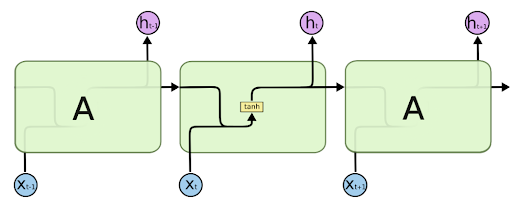
\includegraphics[width=0.7\textwidth]{images/lstm.png}
    \caption{LSTM (Long Short-Term Memory) básico.}
    \label{fig:lstm}
\end{figure}

\begin{itemize}
    \item \textbf{Transformers}: arquitectura inicialmente desarrollada para procesamiento de lenguaje natural, que ha comenzado a aplicarse con éxito en predicción multivariada de series temporales \parencite{li2019}.
\end{itemize}

La elección del modelo dependerá del tipo de datos disponibles, la granularidad deseada y los requisitos de interpretabilidad y precisión. En este proyecto, estos modelos permitirán estimar con mayor exactitud la demanda diaria de productos, reduciendo mermas y ajustando la producción a las condiciones reales del entorno.

\subsection{Evaluación de Modelos Predictivos}

La evaluación de modelos predictivos es un paso fundamental en el desarrollo de soluciones basadas en inteligencia artificial o series temporales, ya que permite medir cuán precisas y útiles son las predicciones generadas. Para problemas de regresión —como la predicción de demanda— se utilizan principalmente métricas de error que comparan los valores predichos con los observados.

Entre las más utilizadas se encuentran:

\begin{itemize}
    \item \textbf{MAE (Mean Absolute Error)}: mide el promedio de los errores absolutos entre las predicciones $\hat{y}_t$ y los valores reales $y_t$ \parencite{willmott2005}.
    
    \[
        \text{MAE} = \frac{1}{n} \sum_{t=1}^{n} \left| y_t - \hat{y}_t \right|
    \]

    \item \textbf{RMSE (Root Mean Squared Error)}: calcula la raíz cuadrada del promedio de los errores al cuadrado, penalizando más fuertemente los errores grandes \parencite{chai2014}.
    
    \[
        \text{RMSE} = \sqrt{ \frac{1}{n} \sum_{t=1}^{n} \left( y_t - \hat{y}_t \right)^2 }
    \]

    \item \textbf{MAPE (Mean Absolute Percentage Error)}: expresa el error como un porcentaje del valor real. Es útil para comparar modelos en distintas escalas, aunque puede ser inestable cuando $y_t \approx 0$ \parencite{myttenaere2016}.
    
    \[
        \text{MAPE} = \frac{100}{n} \sum_{t=1}^{n} \left| \frac{y_t - \hat{y}_t}{y_t} \right|
    \]
\end{itemize}

La elección de la métrica depende del contexto. El MAE es más interpretable para usuarios no técnicos, mientras que el RMSE resulta más sensible a errores significativos. En el caso de predicción de demanda para comercios de productos perecederos, se recomienda utilizar al menos dos métricas para una evaluación equilibrada.

Estas herramientas también permiten monitorear el desempeño del modelo en producción, facilitando el mantenimiento de su precisión a lo largo del tiempo.

\subsection{Reconocimiento Óptico de Caracteres (OCR)}

\indent El Reconocimiento Óptico de Caracteres (OCR) es una tecnología que permite convertir texto impreso o manuscrito en imágenes digitales en texto editable y procesable por máquinas. Es ampliamente utilizada en tareas como la digitalización de documentos, la lectura automatizada de facturas, tickets, formularios y libros (Smith, 2007).

\indent Inicialmente, los sistemas OCR se basaban en técnicas de procesamiento de imágenes y plantillas estáticas, lo que limitaba su capacidad para adaptarse a diferentes formatos, caligrafías o niveles de ruido. Sin embargo, los avances en aprendizaje profundo han revolucionado esta tecnología: los modelos actuales, como CRNN (Convolutional Recurrent Neural Network) y los basados en transformers como TrOCR, ofrecen una mayor precisión y robustez en entornos no estructurados, como fotos tomadas con teléfonos móviles o documentos parcialmente dañados (Baek et al., 2019; Li et al., 2021).

\indent El OCR es especialmente valioso en contextos donde los usuarios no pueden o no desean realizar carga manual de datos, como en pequeños comercios. Al automatizar la lectura de registros de venta o remitos mediante fotos, se reduce la carga operativa y se mejora la calidad del dato ingresado (Khandelwal et al., 2020).

\indent En este proyecto, el OCR cumple un rol clave al permitir a los comerciantes digitalizar información histórica de ventas sin conocimientos técnicos, usando simplemente una fotografía desde la plataforma web, lo cual democratiza el acceso a herramientas de predicción.


\subsection{Modelos de Lenguaje Extensos (LLM)}

\indent Los Modelos de Lenguaje Extensos (Large Language Models, LLM) son un tipo avanzado de modelo de IA entrenado con enormes cantidades de texto para comprender, generar y manipular lenguaje natural de forma coherente y contextual. Se basan en arquitecturas como transformers, que han demostrado ser altamente eficaces para tareas complejas de procesamiento del lenguaje natural (Vaswani et al., 2017).

\indent Los LLM aprenden a predecir la siguiente palabra en una secuencia, lo que les permite ejecutar tareas como generación de texto, traducción, resumen automático, respuestas a preguntas y análisis semántico. Modelos como GPT-3, PaLM, BERT o LLaMA han alcanzado niveles de rendimiento cercanos al humano en una variedad de benchmarks lingüísticos (Brown et al., 2020; OpenAI, 2023).

\indent Una de las aplicaciones emergentes de los LLM es su integración con otros flujos de datos no estructurados, como imágenes o documentos escaneados, lo que los convierte en una herramienta poderosa para la automatización de tareas que antes requerían intervención humana. En combinación con OCR y pipelines de extracción, los LLM pueden interpretar textos ambiguos, corregir errores y convertir inputs visuales en información estructurada (Touvron et al., 2023).

\indent En el contexto de este proyecto, los LLM permiten automatizar la carga de registros de ventas a partir de imágenes, interpretar consultas del usuario en lenguaje natural a través de un chatbot y ofrecer respuestas explicativas, todo sin requerir conocimientos técnicos del usuario final.

\subsection{Chatbots Conversacionales}

Los chatbots conversacionales son sistemas informáticos diseñados para interactuar con los usuarios mediante lenguaje natural, ya sea por texto o voz. Su objetivo principal es simular una conversación humana para asistir, informar, resolver consultas o ejecutar acciones específicas dentro de una plataforma digital \parencite{radziwill2017}.

Originalmente basados en reglas fijas y árboles de decisión, los chatbots han evolucionado significativamente gracias a los avances en procesamiento de lenguaje natural (PLN), generación de lenguaje natural (GNL) y, más recientemente, en modelos de lenguaje extensos (LLM). Estas tecnologías les permiten comprender intenciones, responder con mayor coherencia y adaptarse al contexto de las interacciones \parencite{shum2018}.

Existen distintos tipos de chatbots, entre ellos:

\begin{itemize}
    \item \textbf{Chatbots basados en reglas}: operan sobre flujos de conversación predefinidos.
    
    \item \textbf{Chatbots con IA}: utilizan algoritmos de aprendizaje automático, PLN y GNL para entender y generar respuestas dinámicas.
    
    \item \textbf{Chatbots híbridos}: combinan ambos enfoques, lo que los hace flexibles y eficientes.
\end{itemize}

En aplicaciones empresariales, los chatbots se utilizan cada vez más para consultas sobre datos, gestión de operaciones y soporte a decisiones, especialmente en entornos con usuarios no técnicos. Estudios recientes demuestran que la incorporación de asistentes conversacionales mejora la adopción de sistemas analíticos complejos, reduce barreras de entrada y mejora la experiencia del usuario \parencite{knote2021}.

En este proyecto, el chatbot actuará como interfaz principal del sistema, permitiendo al comerciante consultar predicciones de demanda, indicadores clave (KPIs), alertas de sobreproducción y sugerencias de acción, sin necesidad de navegar por menús complejos ni interpretar gráficos técnicos.

\subsection{Bases de Datos Relacionales y Vectoriales}

Las bases de datos relacionales (RDB, por sus siglas en inglés) son estructuras de almacenamiento que organizan la información en tablas con filas y columnas, siguiendo un modelo basado en el álgebra relacional, propuesta por Edgar F. Codd en 1970. Este modelo formaliza las operaciones sobre conjuntos de datos utilizando el concepto de relación, y se convirtió en el estándar dominante para almacenar información estructurada en sistemas informáticos \parencite{codd1970}. 

Las bases relacionales permiten realizar consultas complejas mediante lenguajes como SQL y son ampliamente utilizadas en aplicaciones empresariales debido a su robustez, integridad referencial y facilidad de acceso \parencite{coronel2020}.

En contraposición, las bases de datos vectoriales son un tipo más reciente de almacenamiento orientado a datos no estructurados o semiestructurados representados como tensores. Su principal aplicación está en sistemas que utilizan inteligencia artificial, especialmente modelos de lenguaje, visión por computadora y recuperación semántica, donde se requiere comparar elementos no por igualdad exacta, sino por similitud de contexto o significado \parencite{johnson2019}.

Estos vectores se obtienen comúnmente a través de \textit{embeddings} generados por modelos como Word2Vec, BERT o CLIP, y se almacenan en motores especializados como FAISS, Milvus o Pinecone, optimizados para búsquedas por proximidad (\textit{nearest neighbor search}).

En el contexto de este proyecto, las bases relacionales serán utilizadas para almacenar información estructurada como productos, ventas, fechas y predicciones, mientras que las bases vectoriales podrían emplearse en versiones futuras para mejorar el rendimiento del chatbot, permitiéndole recuperar respuestas basadas en similitud semántica entre preguntas y registros históricos o documentación del sistema.

\subsection{Desperdicio de Alimentos}

El desperdicio de alimentos hace referencia a la pérdida de productos aptos para el consumo humano que son descartados, deteriorados o no utilizados en etapas finales de la cadena alimentaria, como la comercialización, el almacenamiento o el consumo doméstico. Se diferencia de la pérdida de alimentos, que ocurre en fases anteriores como la producción, poscosecha o procesamiento \parencite{fao2019}.

A nivel mundial, se estima que alrededor del 17\% de los alimentos disponibles para los consumidores se desperdicia, lo que representa no solo un problema ético y de seguridad alimentaria, sino también una amenaza ambiental por el uso innecesario de recursos como agua, tierra y energía, y la generación de gases de efecto invernadero \parencite{unep2021}.

En Argentina, se pierde o desperdicia el 12{,}5\% de la producción agroalimentaria, lo que equivale a aproximadamente 16 millones de toneladas por año, con consecuencias económicas directas para todos los actores de la cadena de valor \parencite{tiscornia2022}. Particularmente en supermercados, autoservicios y comercios de proximidad, estudios recientes estiman que las pérdidas en categorías frescas superan el 3\% de la facturación, debido a sobreproducción, quiebres de stock, manipulación inadecuada o falta de planificación \parencite{weteam2021}.

Estas cifras revelan la importancia de implementar soluciones basadas en inteligencia artificial y analítica de datos para alinear la producción con la demanda real, evitar el sobrante no comercializable y aumentar la eficiencia operativa. Además, el combate al desperdicio de alimentos contribuye directamente al cumplimiento del Objetivo de Desarrollo Sostenible (ODS) 12: Producción y Consumo Responsables, propuesto por la ONU para 2030.

\subsection{Impacto Económico del desperdicio de alimentos}

El desperdicio de alimentos no solo representa una pérdida de recursos naturales y energéticos, sino también un impacto económico significativo para productores, distribuidores, comercios y consumidores. En cada etapa de la cadena alimentaria, los alimentos descartados implican costos hundidos en insumos, mano de obra, energía, logística y espacio, sin retorno económico alguno \parencite{gustavsson2011}.

A nivel global, se estima que el valor económico del desperdicio asciende a 1 billón de dólares anuales, afectando tanto a países desarrollados como en desarrollo \parencite{fao2013}. En entornos urbanos y comerciales, las pérdidas se concentran especialmente en productos frescos y perecederos —como panificados, frutas, carnes y lácteos— debido a errores de planificación, sobreproducción, fluctuaciones de demanda o una gestión ineficiente de inventarios \parencite{fao2019}.

En Argentina, estudios sectoriales revelan que las pérdidas en supermercados y autoservicios superan el 3\% de la facturación en categorías de frescos y almacén, representando un margen crítico para negocios con alta rotación y baja rentabilidad unitaria \parencite{weteam2021}. En comercios pequeños, como panaderías y pastelerías, esta ineficiencia se ve agravada por la falta de herramientas analíticas y predictivas que permitan anticipar la demanda real, provocando mermas frecuentes y subutilización de insumos.

El impacto económico también afecta a escala sistémica: cada tonelada de alimento desperdiciado implica no solo una pérdida directa, sino también costos ocultos en la cadena logística, residuos, tratamiento y emisiones \parencite{refed2016}. Desde esta perspectiva, el desarrollo de soluciones tecnológicas que minimicen el desperdicio contribuye no solo a mejorar la rentabilidad del negocio, sino también a reducir costos operativos y ambientales a largo plazo.

\subsection{Impacto Ambiental del Desperdicio de Alimentos}

El desperdicio de alimentos tiene consecuencias ambientales severas, ya que cada unidad de alimento producida pero no consumida implica un uso innecesario de recursos naturales, como agua, suelo y energía, además de generar residuos y emisiones contaminantes. La huella ambiental del desperdicio incluye tres grandes dimensiones: la huella hídrica, la huella de carbono y el uso del suelo \parencite{fao2013}.

A nivel mundial, se calcula que el desperdicio de alimentos genera entre el 8 y el 10\% de las emisiones globales de gases de efecto invernadero (GEI), lo que equivale a más de 3.300 millones de toneladas de CO\textsubscript{2} emitidas anualmente \parencite{unep2021}. Si el desperdicio de alimentos fuera un país, sería el tercer mayor emisor del mundo, detrás de China y Estados Unidos \parencite{fao2013}.

En cuanto a recursos hídricos, se estima que alrededor de 250~km\textsuperscript{3} de agua se utilizan cada año para producir alimentos que nunca serán consumidos, lo que representa una presión significativa sobre acuíferos y sistemas hídricos vulnerables. Además, el uso ineficiente del suelo para cultivos que luego se pierden contribuye a la deforestación, pérdida de biodiversidad y degradación de ecosistemas \parencite{kummu2012}.

En el caso de Argentina, donde se desperdician más de 16 millones de toneladas de alimentos por año \parencite{tiscornia2022}, el impacto ambiental se agrava por la dependencia del sector agroindustrial como motor económico, lo que exige soluciones que equilibren productividad y sostenibilidad. Reducir el desperdicio, por tanto, no solo mejora la eficiencia de los sistemas alimentarios, sino que también representa una estrategia concreta de mitigación del cambio climático \parencite{unep2021}.

Desde esta perspectiva, el proyecto presentado cobra relevancia al buscar reducir la sobreproducción mediante herramientas de predicción basadas en inteligencia artificial, contribuyendo así a una gestión más sostenible de los recursos.

\subsection{ODS 12 – Producción y Consumo Responsables}

El Objetivo de Desarrollo Sostenible 12 (ODS 12), propuesto por las Naciones Unidas en la Agenda 2030, tiene como meta garantizar modalidades de consumo y producción sostenibles, promoviendo un uso eficiente de los recursos, la energía y los sistemas productivos, sin comprometer las necesidades de las generaciones futuras \parencite{onu2015}.

Uno de los ejes centrales del ODS 12 es la reducción sustancial del desperdicio de alimentos, tanto en la etapa de producción como en los sectores minorista y de consumo. La meta 12.3, en particular, establece como compromiso internacional reducir a la mitad el desperdicio de alimentos per cápita mundial en el comercio minorista y el consumidor para el año 2030, y disminuir las pérdidas a lo largo de las cadenas de producción y suministro \parencite{unep2021}.

Este objetivo reconoce que el desperdicio alimentario es un problema transversal: tiene impactos económicos, sociales (inseguridad alimentaria) y ambientales (emisiones de gases de efecto invernadero, uso de agua y suelo). Por eso, la tecnología juega un rol clave como habilitadora de soluciones innovadoras y escalables, particularmente en el sector privado.

En este contexto, el presente proyecto de ingeniería se alinea directamente con el ODS 12, al proponer una plataforma que utiliza inteligencia artificial para predecir la demanda real en comercios de productos perecederos, evitando sobreproducción y mermas innecesarias. Así, no solo mejora la rentabilidad de los negocios, sino que contribuye a un modelo de producción más eficiente, consciente y responsable con el entorno.

\subsection{Digitalización y brecha tecnológica en PYMEs}

La digitalización implica la incorporación de tecnologías digitales en los procesos productivos, administrativos y comerciales de las organizaciones, con el objetivo de mejorar su eficiencia, competitividad y capacidad de adaptación. Sin embargo, las pequeñas y medianas empresas (PYMEs) enfrentan múltiples barreras estructurales que dificultan su transformación digital, generando una brecha tecnológica creciente respecto de grandes empresas o corporaciones \parencite{oecd2021}.

Entre las principales limitaciones que afectan a las PYMEs se encuentran:

\begin{itemize}
    \item Falta de acceso a infraestructura tecnológica adecuada (hardware, software, conectividad).
    \item Baja disponibilidad de talento digital o personal capacitado.
    \item Costos percibidos como elevados, especialmente en soluciones basadas en IA o big data.
    \item Desconocimiento de herramientas existentes y sus beneficios.
    \item Miedo al cambio o resistencia organizacional \parencite{jordao2022}.
\end{itemize}

En América Latina y particularmente en Argentina, estas brechas son aún más pronunciadas. Estudios del BID señalan que solo 1 de cada 4 PYMEs en la región adopta tecnologías digitales avanzadas, y que más del 60~\% se encuentra en niveles básicos de digitalización \parencite{bid2020}. Complementariamente, un estudio reciente sobre digitalización contable en PYMEs de Ecuador identificó que los principales obstáculos son la falta de capacitación, los altos costos iniciales y la resistencia al cambio, y destacó que el acceso a tecnología, formación profesional y apoyo institucional son determinantes para una adopción exitosa \parencite{vasconez2025}.

Entre sus hallazgos, se estima que la digitalización puede aumentar los ingresos en un 30~\% y reducir los costos operativos en un 20~\%, aunque aún persisten desafíos relacionados con la visión estratégica y el capital disponible.

En el sector alimentario, la falta de herramientas tecnológicas específicas impide a muchos comercios ajustar su producción a la demanda real, generando ineficiencias como sobreproducción, desperdicio o rotura de stock. Por eso, el desarrollo de plataformas accesibles, intuitivas y enfocadas en resolver problemas concretos de gestión —como la que se propone en este proyecto— resulta clave para acortar la brecha digital, profesionalizar la toma de decisiones y mejorar la sostenibilidad operativa de los pequeños comercios.

\chapter{Estado del Arte}\label{chapter03}

La predicción de demanda en comercios que operan con productos perecederos representa un desafío significativo debido a la naturaleza volátil y sensible al tiempo de estos bienes. En las últimas décadas, el avance de las tecnologías de inteligencia artificial y aprendizaje automático ha permitido desarrollar soluciones cada vez más sofisticadas para anticipar patrones de consumo y optimizar la producción, con el objetivo de minimizar pérdidas y mejorar la eficiencia operativa.

Este estado del arte presenta una revisión crítica de las soluciones tecnológicas existentes y los enfoques académicos más relevantes aplicados a la predicción de demanda en el sector alimentario, con especial énfasis en productos frescos y perecederos. Se analizan modelos, métricas y tecnologías empleadas, así como las limitaciones que enfrentan estas soluciones, especialmente en contextos de pequeñas y medianas empresas con restricciones operativas y tecnológicas.

A partir de este análisis, se evidencian las oportunidades y necesidades no cubiertas que motivan el desarrollo de la propuesta de este proyecto, orientada a un contexto local con condiciones económicas y sociales específicas, buscando ofrecer una herramienta accesible, flexible y efectiva para comercios minoristas.

\section{Soluciones Tecnológicas Existentes}

En el mercado global existen diversas soluciones tecnológicas orientadas a la predicción de demanda, particularmente en \textit{retail} alimentario:

\begin{itemize}
    \item \textbf{SAP Forecasting and Replenishment (F\&R)}: solución empresarial para la planificación de inventarios y reposición automática, basada en modelos estadísticos y reglas de negocio. No utiliza inteligencia artificial. Para funcionalidades avanzadas con IA, SAP ofrece una solución distinta llamada \textit{SAP Predictive Replenishment} \parencite{sap2025}.
    
    \item \textbf{Oracle Retail Demand Forecasting}: incorpora algoritmos de aprendizaje automático para analizar variables como estacionalidad, promociones y eventos. Aunque potente, no está orientado a PYMEs y requiere una alta inversión en integración \parencite{oracle2021}.
    
    \item \textbf{BakePlan}: herramienta especializada para panaderías en Europa. Estima cantidades ideales de productos horneados por día usando datos de ventas y clima. Si bien demuestra mejoras en reducción de merma, no es adaptable fuera de entornos regulados y con datos estructurados \parencite{netherlands2019}.
    
    \item \textbf{Blue Yonder Luminate}: plataforma SaaS con capacidades de \textit{forecast} basadas en IA. Apta para grandes superficies, pero inadecuada para comercios sin personal técnico o sin sistemas previos de digitalización.
\end{itemize}

Estos estudios confirman que los modelos neuronales como LSTM y Bi-LSTM superan en precisión a los enfoques clásicos, especialmente en entornos con múltiples variables externas (como el clima), lo que refuerza su aplicabilidad en el presente proyecto.

\section{Estudios y enfoques académicos}

Investigaciones recientes han abordado la predicción de demanda para alimentos perecederos con distintos enfoques:

\begin{itemize}
    \item \textcite{nassibi2023} compararon modelos de \textit{machine learning} (Random Forest, SVM, LSTM) para predecir la demanda en la industria alimentaria. LSTM logró el menor error promedio (RMSE) al capturar patrones temporales no lineales.

    \item \textcite{ni2022} utilizaron un modelo Bi-LSTM para predecir demanda logística en plataformas de \textit{e-commerce} de alimentos frescos. Al incluir variables climáticas y días festivos, lograron reducir el MAE en un 12{,}6\,\% respecto de modelos base.

    \item \textcite{bandara2020} propusieron LSTM-MSNet para predecir múltiples series temporales con patrones estacionales. El modelo superó a Prophet y Holt-Winters al manejar datos ruidosos e incompletos.
\end{itemize}

Estos estudios confirman que los modelos neuronales como LSTM y Bi-LSTM superan en precisión a los enfoques clásicos, especialmente en entornos con múltiples variables externas (como el clima), lo que refuerza su aplicabilidad en el presente proyecto.



\begin{table}[t]
    \centering
    \renewcommand{\arraystretch}{1.3}
    \caption{Comparación de enfoques}
    \label{tab:comparacion}
    \begin{tabular}{|p{2.9cm}|p{2cm}|p{3cm}|p{5cm}|}
        \hline
        \textbf{Modelo / Solución} & \textbf{Tipo} & \textbf{Tecnologías principales} & \textbf{Limitaciones destacadas} \\
        \hline
        SAP F\&R & Comercial & ARIMA, reglas heurísticas & Costoso, complejo \\
        \hline
        Oracle RDF & Comercial & ML + estacionalidad & Requiere datos limpios (MAPE, RMSE) \\
        \hline
        BakePlan & Comercial (PYME) & Reglas, regresiones & No escalable (\% de merma) \\
        \hline
        Nassibi et al. (2023) & Académico & LSTM, Random Forest & No adaptado a Argentina (MAE, RMSE) \\
        \hline
        Ni et al. (2022) & Académico & Bi-LSTM & Datos estructurados (MAE, RMSE) \\
        \hline
        Propuesta actual (PFI) & Académico & LSTM, Prophet, LLMs & Datos limitados iniciales (MAE, RMSE, MAPE) \\
        \hline
    \end{tabular}
\end{table}


\section{Aporte diferencial del proyecto}

El sistema propuesto en este proyecto se distingue de las soluciones analizadas por las siguientes características:

\begin{itemize}
    \item \textbf{Accesibilidad}: pensado específicamente para pequeños comercios argentinos sin sistemas previos de gestión ni personal técnico.

    \item \textbf{Multimodalidad}: permite la carga de registros mediante imágenes, utilizando modelos OCR y LLMs, lo cual no está presente en las herramientas comerciales revisadas.

    \item \textbf{Interfaz natural}: reemplaza los paneles tradicionales por un chatbot conversacional en lenguaje natural, facilitando el uso incluso por usuarios no técnicos.

    \item \textbf{Costo operativo bajo}: arquitectura liviana, adaptable, y con un presupuesto estimado de solo USD~50 mensuales.

    \item \textbf{Orientación local}: los modelos se entrenan considerando variables específicas como clima y feriados de Buenos Aires en el año 2025.
\end{itemize}



	\chapter{Descripción}\label{chapter03}

AIVA es un sistema web orientado a pequeñas y medianas empresas de alimentos perecederos, como por ejemplo panaderías y confiterías, que busca reducir mermas y quiebres de stock mediante la planificación de producción y reposición basada en datos. La propuesta integra, en una única plataforma, la captura flexible de ventas (punto de venta, importación de CSV y carga asistida por imágenes), el enriquecimiento contextual (clima, calendario y patrones semanales) y un módulo de predicción de demanda diaria por producto. Sobre esta base, el sistema ofrece visualizaciones ejecutivas (backoffice), un asistente conversacional para consultas operativas y un mecanismo de alertas que anticipa situaciones de sobreproducción o faltantes. 

El núcleo analítico del sistema combina el historial transaccional con variables exógenas para estimar la demanda esperada a corto plazo. Este módulo implementa un enfoque heurístico transparente centrado en tendencia, estacionalidad y condiciones meteorológicas, con un diseño abierto a la incorporación de modelos estadísticos y de aprendizaje automático más avanzados. La arquitectura prioriza componentes de bajo costo y rápida adopción, asegurando trazabilidad de datos, reproducibilidad de resultados y una experiencia de usuario alineada con los flujos cotidianos del negocio.


\vspace{1cm}
\section{Requerimientos del sistema}
Esta sección especifica las condiciones verificables que delimitan el alcance de AIVA. Se formulan en modo imperativo (“El sistema debe …”) para facilitar su prueba y aceptación. Se organizan en dos grupos: funcionales (capacidades observables) y no funcionales (calidades y restricciones transversales).

\subsection{Requerimientos funcionales}
Definen lo que el sistema hace de cara al usuario y a los procesos de negocio (captura de datos, análisis y presentación). Recogen sólo lo esencial para operar AIVA extremo a extremo, sin imponer detalles de implementación.

\begin{enumerate}[label=RF-\arabic*., leftmargin=*, nosep]
  \item El sistema debe permitir registro, verificación de correo e inicio/cierre de sesión.
  \item El sistema debe asignar automáticamente un plan gratuito al alta y reflejarlo en la sesión.
  \item El sistema debe mantener la sesión activa y renovar credenciales mientras sean válidas.
  \item El sistema debe gestionar productos y categorías con operaciones CRUD.
  \item El sistema debe permitir cargar productos y ventas históricas vía CSV con validación previa.
  \item El sistema debe registrar ventas mediante un flujo POS con totales e ítems por producto.
  \item El sistema debe enriquecer transacciones con contexto (fecha, día, clima, feriados/fin de semana).
  \item El sistema debe generar predicciones de demanda por producto considerando tendencia, estacionalidad y clima.
  \item El sistema debe asociar a cada predicción nivel de confianza, factores explicativos y recomendación de stock.
  \item El sistema debe persistir predicciones por usuario y período y permitir su recalculo bajo demanda.
  \item El sistema debe exponer un tablero con KPIs de ventas, clima y predicciones vigentes.
  \item El sistema debe ofrecer un asistente conversacional para consultas y navegación guiada (\texttt{/api/chat}).
  \item El sistema debe generar y listar alertas operativas (stock bajo, sobreproducción potencial, feriados).
  \item El sistema debe filtrar todos los datos por el identificador del usuario autenticado.
\end{enumerate}

\subsection{Requerimientos no funcionales}
Establecen cualidades globales del sistema (seguridad, desempeño, mantenibilidad, confiabilidad). Limitan cómo se implementan los servicios, sin modificar el comportamiento funcional.

\begin{enumerate}[label=RNF-\arabic*., leftmargin=*, nosep]
  \item El sistema debe proteger recursos con autenticación/autorización y transmitir credenciales sólo por HTTPS.
  \item El sistema debe aplicar segmentación de datos en base (RLS o equivalente) por \texttt{user\_id}.
  \item El sistema debe ofrecer tiempos de respuesta percibidos menores a 2\,segundos en navegación del \textit{dashboard}.
  \item El sistema debe calcular predicciones bajo demanda en tiempos compatibles con uso interactivo (orden de segundos).
  \item El sistema debe manejar entradas inválidas y fallas externas con mensajes categorizados y recuperables.
  \item El sistema debe registrar eventos relevantes (errores, importaciones, cálculos) para auditoría.
  \item El sistema debe ser usable en navegadores modernos de escritorio y responder correctamente en distintos anchos.
  \item El sistema debe cumplir pautas básicas de accesibilidad (contraste, etiquetas/ARIA en controles principales).
  \item El sistema debe preservar integridad referencial y usar transacciones en altas de ventas.
  \item El sistema debe favorecer mantenibilidad con módulos tipados y convenciones de estilo consistentes.
  \item El sistema debe gestionar secretos vía variables de entorno y rotar credenciales periódicamente.
  \item El sistema debe respetar privacidad aplicable, realizar respaldos de datos críticos y versionar migraciones.
\end{enumerate}

\vspace{1cm}
\section{Historias de usuario}
Esta sección captura, en lenguaje natural, necesidades y objetivos de los actores del sistema. Cada historia sigue el formato \emph{«Como [rol], quiero [objetivo] para [beneficio]»} e incluye criterios de aceptación sintéticos.

\begin{enumerate}[label=HU-\arabic*., leftmargin=*, nosep]

\item Como \textbf{Comerciante nuevo}, quiero registrarme e iniciar sesión con verificación de correo para comenzar a usar AIVA de forma segura.
\begin{itemize}[nosep]
\item No se permite acceso hasta confirmar el correo; al confirmar, queda sesión activa.
\item Tras el alta, se asigna automáticamente el plan gratuito y se refleja en la sesión.
\end{itemize}

\item Como \textbf{Comerciante}, quiero fijar mi ubicación por defecto para que el sistema incorpore clima local en análisis y predicciones.
\begin{itemize}[nosep]
\item La ubicación se persiste y es editable por el usuario.
\item Las consultas al servicio de clima usan la ubicación guardada.
\end{itemize}

\item Como \textbf{Administrador de catálogo}, quiero gestionar productos y categorías (crear/editar/eliminar) para mantener actualizado el inventario.
\begin{itemize}[nosep]
\item Validación de campos obligatorios y unicidad por usuario.
\item Historial de movimientos de stock visible por producto.
\end{itemize}

\item Como \textbf{Administrador de catálogo}, quiero cargar productos por CSV con vista previa para acelerar altas masivas sin errores.
\begin{itemize}[nosep]
\item Se validan columnas mínimas; se muestra resumen de aceptadas/rechazadas.
\item La importación es idempotente y permite revertir en caso de error.
\end{itemize}

\item Como \textbf{Cajero/a}, quiero registrar una venta tipo POS con carrito y totales para asentar transacciones rápidamente.
\begin{itemize}[nosep]
\item La confirmación crea venta e ítems de forma atómica y actualiza stock.
\item La transacción queda enriquecida con fecha/día y banderas de contexto.
\end{itemize}

\item Como \textbf{Analista}, quiero importar ventas históricas (CSV) para consolidar el histórico que alimenta reportes y predicciones.
\begin{itemize}[nosep]
\item Normalización de fechas/productos y registro descargable de errores.
\item Detección de duplicados para evitar dobles cargas (idempotencia).
\end{itemize}

\item Como \textbf{Operador}, quiero registrar ventas asistidas por imágenes (OCR) para acelerar la carga desde comprobantes.
\begin{itemize}[nosep]
\item Estados visibles: en cola, procesando, listo; notificación al completar.
\item Edición/corrección antes de confirmar el alta definitiva.
\end{itemize}

\item Como \textbf{Responsable de producción}, quiero ver y recalcular predicciones (hoy/semana/mes) para planificar elaboración y reposición.
\begin{itemize}[nosep]
\item Cada predicción incluye confianza, factores y recomendación de stock.
\item Se persisten por fecha/usuario y se marcan como vigentes.
\end{itemize}

\item Como \textbf{Encargado}, quiero recibir alertas de quiebre/sobreproducción y feriados para actuar preventivamente.
\begin{itemize}[nosep]
\item Listado priorizado por criticidad con fecha y producto.
\item Enlaces a la acción sugerida (ajuste de producción/stock).
\end{itemize}

\item Como \textbf{Gerente}, quiero un \textit{dashboard} y reportes por período, producto y categoría para monitorear desempeño y tendencias.
\begin{itemize}[nosep]
\item Gráficos comparan observado vs.\ predicho con filtros persistentes.
\item Exportes básicos (tabla/gráfico) para análisis externo.
\end{itemize}

\item Como \textbf{Usuario}, quiero consultar al asistente conversacional para obtener métricas y ejecutar tareas frecuentes sin salir del flujo.
\begin{itemize}[nosep]
\item Gestión de conversaciones (crear/cambiar/archivar) y copia de respuestas.
\item Manejo de errores categorizado y posibilidad de cancelar la respuesta.
\end{itemize}

\item Como \textbf{Usuario de plan gratuito}, quiero poder adquirir una suscripción desde la app para habilitar capacidades avanzadas.
\begin{itemize}[nosep]
\item Verificación de identidad y confirmación de pago cuando corresponda.
\item La nueva capacidad se refleja de inmediato en la sesión.
\end{itemize}

\end{enumerate}


\vspace{1cm}
\section{Interfaz gráfica}
En esta sección se expone la interfaz gráfica desarrollada para la interacción cotidiana de los usuarios de AIVA en el entorno de comercio minorista de alimentos perecederos. La UI prioriza baja fricción operativa, consistencia visual y señales claras para la toma de decisiones, con patrones reutilizables que reducen la curva de aprendizaje. A continuación se describen las dos pantallas más relevantes por su impacto en el trabajo diario: el asistente conversacional (chatbot) y el módulo de predicción de demanda.

\subsection{Asistente conversacional (chatbot)}
\begin{figure}[!htbp]
  \centering
  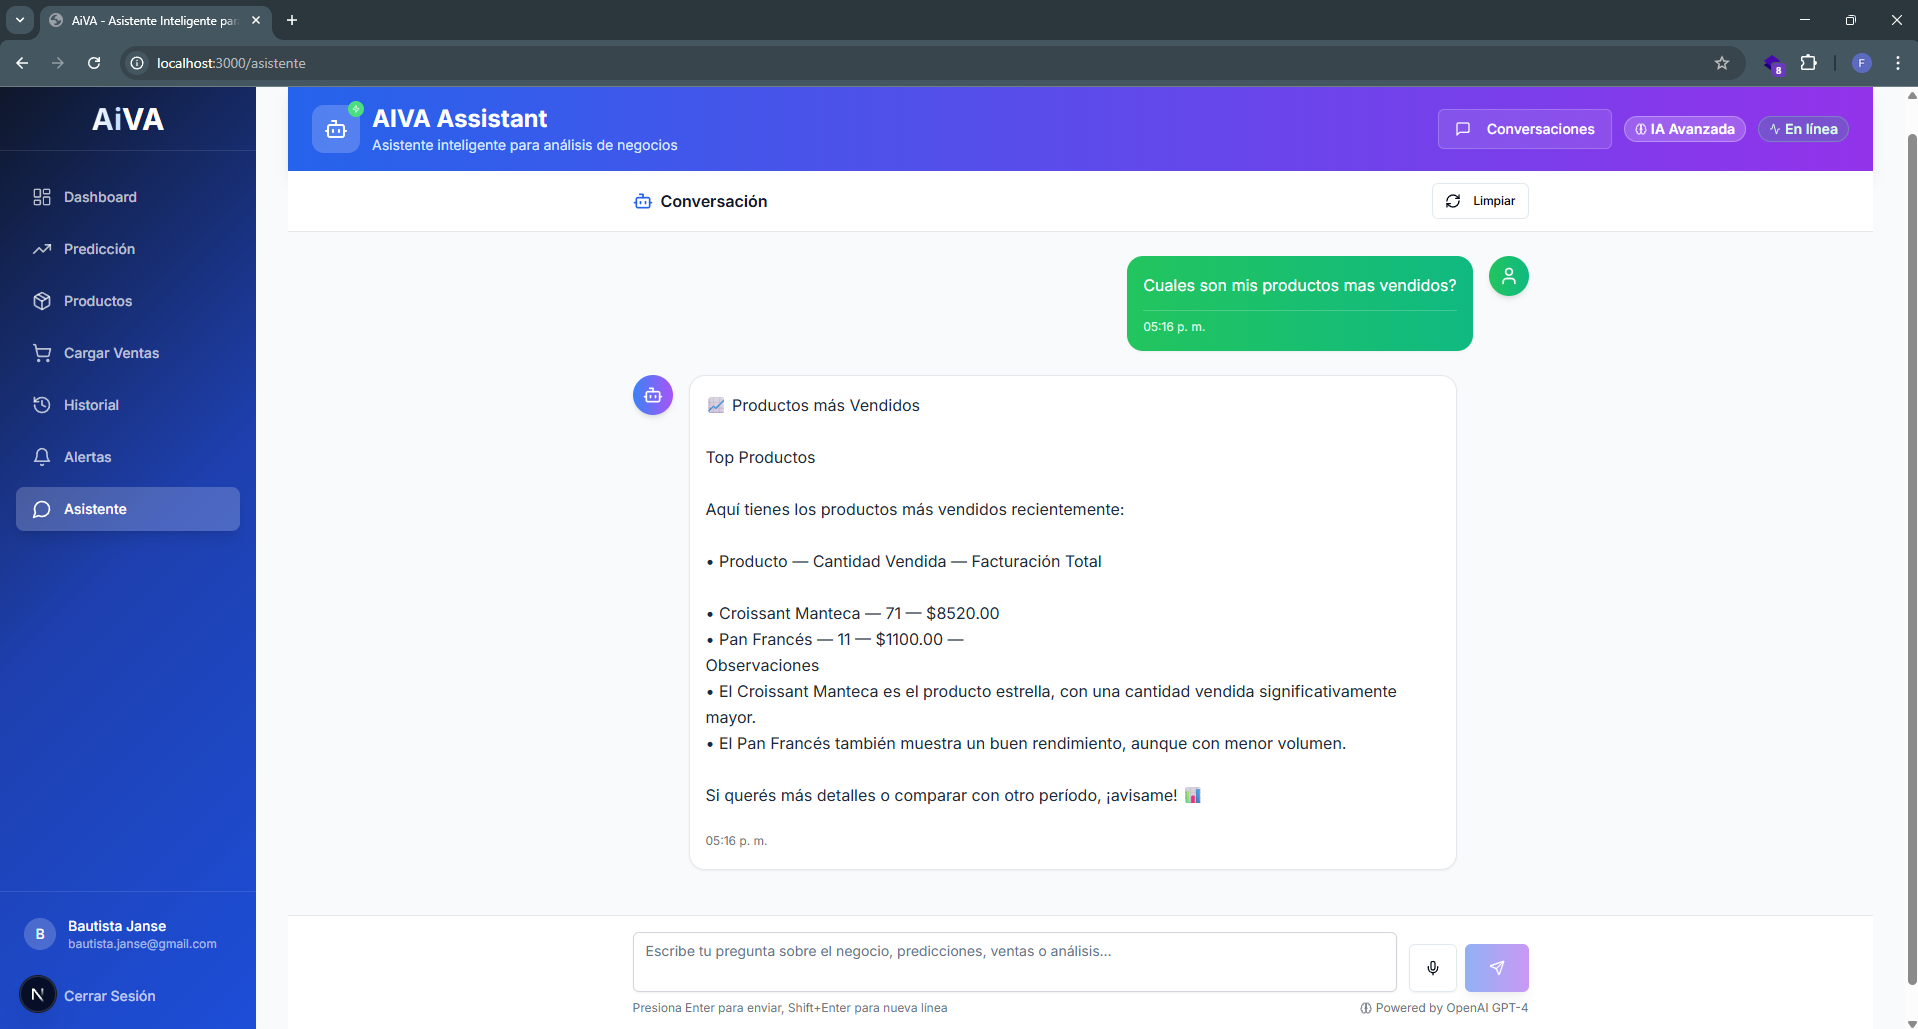
\includegraphics[width=0.92\textwidth]{images/chatbotPage.png}
  \caption{Asistente conversacional (chatbot) -- Fuente: elaboración propia}
  \label{fig:ui-chatbot}
\end{figure}
La pantalla del asistente provee un canal de interacción en lenguaje natural para consultar métricas, navegar a vistas operativas y disparar acciones frecuentes sin abandonar el flujo de trabajo. El encabezado, con gradiente azul–violeta, muestra el estado del servicio mediante la insignia («En línea») y un selector de conversaciones que permite crear, cambiar y archivar hilos, favoreciendo la continuidad y la trazabilidad de consultas.

El área central es un historial desplazable con burbujas alineadas según el rol: los mensajes del usuario se muestran a la derecha y las respuestas del asistente, a la izquierda. Cada mensaje incorpora marca de tiempo y, en el caso del asistente, una acción para copiar el contenido. Cuando no hay historial, se presenta un saludo dinámico según la hora y atajos de acción (“Ver predicciones de mañana”, “Analizar ventas de esta semana”) que precargan consultas típicas para reducir fricción.

La barra inferior concentra la entrada de texto, con envío por Enter y salto de línea con \textit{Shift+Enter}, y botones para enviar o limpiar la conversación. Durante el procesamiento se indica actividad y se habilita la interrupción segura de la respuesta. La comunicación con el backend se realiza autenticada (token de sesión de Supabase) contra el endpoint interno \texttt{/api/chat}; se contemplan estados de error categorizados (cuota, servicio, autenticación, cancelación y red) con retroalimentación visual y mensajes recuperables. En conjunto, el diseño prioriza velocidad de uso, consistencia con el resto de la interfaz y control explícito sobre el ciclo de la conversación.

\subsection{Procesamiento de la consulta}
Cuando el usuario ingresa una consulta en el chat, el asistente procesa el mensaje y determina la intención de la pregunta a partir del lenguaje natural. En lugar de devolver una respuesta predefinida o aproximada, el agente genera de manera dinámica una consulta SQL parametrizada que traduce esa necesidad en una instrucción concreta sobre la base de datos. Esta consulta, siempre restringida a operaciones de solo lectura y filtrada por el identificador del usuario, se ejecuta en Supabase sobre el motor Postgres, garantizando seguridad y acceso únicamente a la información correspondiente. Una vez obtenidos los resultados, el asistente procesa los datos para calcular métricas, agrupar valores y elaborar indicadores relevantes, que luego son redactados en un formato comprensible y ejecutivo. De esta manera, el usuario recibe una respuesta clara y contextualizada, sustentada en datos reales y actualizados, sin exposición de detalles técnicos. El enfoque adoptado constituye el núcleo innovador de la solución: transformar de forma automática las consultas en lenguaje natural en consultas SQL seguras, ejecutarlas en tiempo real y presentar los resultados de manera amigable dentro del flujo conversacional.

\subsection{Predicción de demanda}
\begin{figure}[!htbp]
\centering
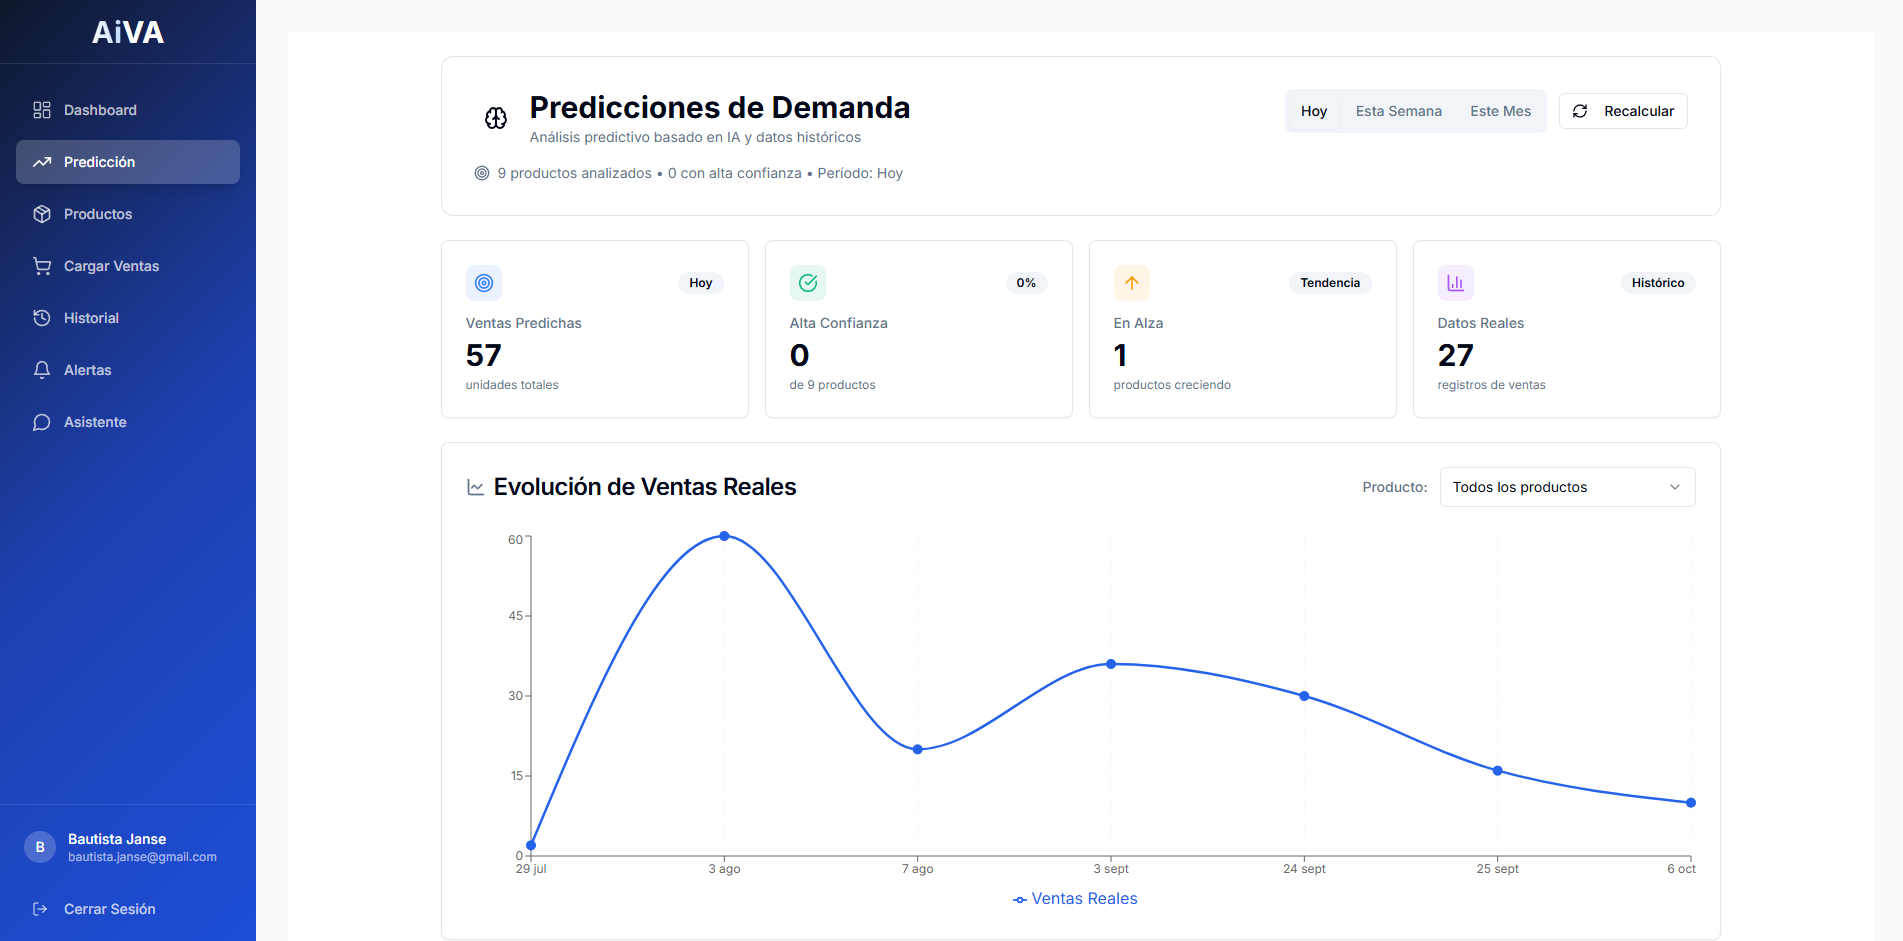
\includegraphics[width=0.95\textwidth]{images/prediccionPage.png}
\caption{Predicción de demanda -- Fuente: elaboración propia}
\label{fig:ui-prediccion}
\end{figure}
La pantalla de predicción concentra el cálculo y la consulta de estimaciones por producto. El encabezado permite elegir el período de análisis (hoy, semana, mes) y recalcular bajo demanda; al mismo tiempo, resume el estado del proceso con indicadores clave (ventas predichas, confianza alta, tendencia positiva y volumen de datos históricos). La sección analítica combina un gráfico de ventas reales filtrable por producto con tres vistas complementarias: un resumen ejecutivo (top productos y riesgos), un detalle tabular con filtros por producto/categoría y umbral de confianza, y un historial de ventas con contexto (clima, fin de semana, feriados). Las predicciones se generan en tiempo real mediante el servicio de predicción y se persisten en la base (tabla \texttt{predictions}, por usuario y período), priorizando trazabilidad, consistencia visual con el dashboard y manejo explícito de errores/estados para decisiones operativas rápidas.

\subsection{Procesamiento de prediccón}
Cuando se registra una venta en el sistema, además de almacenar la transacción, se capturan variables contextuales relevantes como fecha y hora, condiciones climáticas, feriados y características del producto (por ejemplo, si es perecedero). Estos datos se combinan con el historial reciente de ventas para estimar la demanda futura de cada producto, aplicando factores de tendencia, estacionalidad y contexto temporal. El resultado de este proceso es una predicción por período (hoy, semana o mes) que incluye métricas de cantidad esperada, nivel de confianza, tendencia y recomendaciones de stock. Las predicciones generadas se guardan automáticamente en la base de datos en la tabla \texttt{predictions}, asociadas al usuario y al período, lo que asegura que luego puedan ser consultadas en tiempo real desde la interfaz conversacional o visualizadas en la pantalla analítica. De este modo, cada nueva venta no solo actualiza el registro histórico, sino que alimenta y refina las estimaciones disponibles para la toma de decisiones.


\section{Tecnologías utilizadas}\label{sec:tecnologias}
A continuación se detallan las tecnologías empleadas en AIVA, explicando su rol dentro de la solución, el modo de integración y los criterios que justifican su elección. La selección prioriza un balance entre rapidez de implementación, bajo costo operativo, mantenibilidad y adecuación a los requerimientos del sistema.

\subsection{Next.js (React + TypeScript)}
Next.js es un \textit{framework} sobre React que incorpora enrutamiento, optimizaciones de rendimiento y opciones de renderizado (cliente/servidor). En AIVA se utiliza para:
\begin{itemize}
    \item Implementar la interfaz web con componentes reutilizables y tipado estático (TypeScript), reduciendo defectos en tiempo de compilación.
    \item Organizar el ruteo (App Router) separando vistas operativas (\textit{dashboard}, POS, predicción, reportes) de páginas auxiliares (autenticación, perfil).
    \item Favorecer una arquitectura mantenible (módulos, \textit{hooks} y servicios) con buena escalabilidad del frontend.
\end{itemize}
\noindent\textbf{Motivación.} Ecosistema maduro y documentación extensa, compatible con librerías modernas de UI.

\subsection{Tailwind CSS y \textit{shadcn/ui}}
Tailwind CSS provee utilidades de estilo de bajo nivel; \textit{shadcn/ui} aporta componentes accesibles basados en Tailwind.
\begin{itemize}
    \item Permiten maquetar formularios, tablas, modales y gráficos con consistencia visual y tiempos de desarrollo acotados.
    \item Estandarizan patrones de interacción (validaciones, estados de carga y error) y facilitan la personalización fina del diseño.
\end{itemize}
\noindent\textbf{Motivación.} Coherencia visual y productividad. 

\subsection{Recharts}
Recharts es una biblioteca de gráficos para React.
\begin{itemize}
    \item Se utiliza en el \textit{dashboard} y reportes para visualizar KPIs (ventas por período, productos destacados) y comparativas (predicción vs.\ observado).
    \item Ofrece componentes responsivos y composables, adecuados para vistas con filtros interactivos.
\end{itemize}
\noindent\textbf{Motivación.} Integración directa con React y bajo costo de aprendizaje.

\subsection{Supabase Auth}
Servicio gestionado para registro, inicio de sesión y manejo de sesiones (incluida verificación por correo).
\begin{itemize}
    \item Centraliza la identidad del usuario y emite \textit{tokens} para acceder a recursos protegidos.
    \item Simplifica la implementación de rutas seguras y del \textit{feature gating} por plan/suscripción.
\end{itemize}
\noindent\textbf{Motivación.} Reduce superficie de error y esfuerzo de mantenimiento respecto de una solución propia.

\subsection{PostgreSQL (vía Supabase)}
Base de datos relacional donde reside el modelo de datos.
\begin{itemize}
    \item Tablas operativas: \texttt{products}, \texttt{categories}, \texttt{sales}/\texttt{sale\_items}, \texttt{stock\_movements}.
    \item Datos analíticos y de contexto: \texttt{demand\_analysis\_data}, \texttt{predictions}/\texttt{stored\_predictions}, \texttt{weather\_data}, \texttt{plans}, \texttt{user\_subscriptions}.
    \item Soporte de integridad referencial, vistas e \textit{indexes} para consultas eficientes.
\end{itemize}
\noindent\textbf{Motivación.} Robustez y expresividad SQL para analítica operativa.

\subsection{PostgREST (Supabase)}
Capa que expone el esquema de PostgreSQL como API REST tipada.
\begin{itemize}
    \item La capa de servicios del frontend consume esta API para operaciones CRUD y consultas filtradas.
    \item Mantiene trazabilidad entre el modelo lógico y los endpoints, reduciendo código \textit{boilerplate}.
\end{itemize}
\noindent\textbf{Motivación.} Acelera la construcción de la capa de datos manteniendo convenciones REST.

\subsection{OpenWeatherMap API}
Fuente externa de variables meteorológicas usadas como factores exógenos.
\begin{itemize}
    \item Proporciona temperatura, estado del tiempo y otros atributos que se asocian a ventas y se persisten para análisis.
    \item Se contemplan \textit{fallbacks} ante indisponibilidad o latencia elevada.
\end{itemize}
\noindent\textbf{Motivación.} Cobertura suficiente para el ámbito del proyecto.

\subsection{Node.js y npm}
Entorno de ejecución y gestor de dependencias del proyecto.
\begin{itemize}
    \item Se emplea para el servidor de desarrollo, construcción del frontend y automatización de tareas (scripts).
    \item Estandariza \textit{linting}, empaquetado y gestión de versiones.
\end{itemize}
\noindent\textbf{Motivación.} \textit{Tooling} ampliamente adoptado en el ecosistema web.

\subsection{Utilitarios de CSV}
Conjunto de utilidades para ingesta histórica.
\begin{itemize}
    \item Validan formato, normalizan columnas y registran errores durante la carga de productos y ventas.
    \item Priorizan trazabilidad (filas aceptadas, rechazadas o corregidas) para reproducibilidad.
\end{itemize}
\noindent\textbf{Motivación.} Simplicidad y compatibilidad con exportaciones comunes.

\subsection{Buenas prácticas de configuración y seguridad}
\begin{itemize}
    \item Gestión de credenciales mediante variables de entorno (\texttt{.env}), evitando su versionado.
    \item Separación de entornos (desarrollo/producción) y rotación periódica de claves.
    \item En despliegues gestionados, aplicación de RLS por \textit{user\_id} para segmentación de datos.
\end{itemize}




\section{Arquitectura del sistema}

La arquitectura adoptada se basa en un modelo de tres capas 
(presentación, lógica de negocio y persistencia), apoyada en 
servicios gestionados para simplificar la operación y garantizar 
escalabilidad. El diseño busca un equilibrio entre simplicidad 
en el desarrollo y robustez en la operación, integrando 
componentes internos con servicios externos especializados.

\subsection{Capa de presentación (Front-end)}

La interfaz de usuario está implementada en \textbf{Next.js}, que cumple un doble rol:
\begin{itemize}
    \item Renderizado del front-end (formularios, dashboards, carga de datos).
    \item Exposición de endpoints internos (/api) que conectan directamente con los servicios del backend.
\end{itemize}

Los usuarios interactúan con el sistema a través de esta capa 
para gestionar productos, registrar ventas, consultar predicciones 
y atender alertas. Todas las solicitudes son enviadas al backend 
con los \textit{tokens JWT} emitidos por el servicio de autenticación.

\subsection{Capa de lógica de negocio (Backend + API Services)}

El backend, desarrollado en \textbf{Node.js}, centraliza la lógica de negocio. 
Está organizado en servicios que exponen distintos endpoints específicos.

El backend también se encarga de la validación de datos, el control 
de acceso mediante los JWT emitidos por Supabase Auth, y la interacción 
con la base de datos.

\subsection{Capa de datos (Supabase)}

La persistencia está gestionada por \textbf{Supabase}, que provee:
\begin{itemize}
    \item Base de datos PostgreSQL para almacenar usuarios, productos, ventas, predicciones y alertas.
    \item Módulo de autenticación (\textit{Supabase Auth}), encargado de la provisión y validación de tokens JWT, con \textit{Row Level Security (RLS)} configurado para restringir el acceso por \texttt{user\_id}.
\end{itemize}

La comunicación entre backend y Supabase se realiza a través de 
consultas SQL, garantizando consistencia y trazabilidad de los datos.

\subsection{Integraciones externas}

El sistema se enriquece con dos servicios externos:
\begin{itemize}
    \item \textbf{OpenWeather}: fuente de datos meteorológicos (temperatura, precipitaciones, condiciones climáticas) que son integrados al proceso de predicción de la demanda.
    \item \textbf{OpenAI}: utilizado tanto para el asistente conversacional como para procesos de OCR avanzado, ampliando la capacidad de interacción y automatización del sistema.
\end{itemize}


\begin{figure}[!htbp]
  \centering
  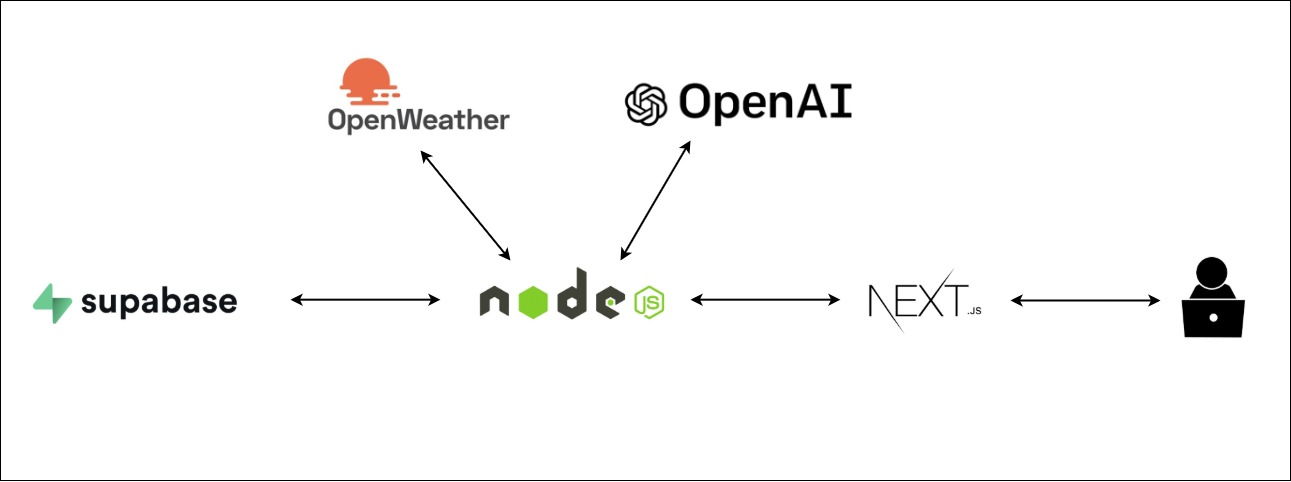
\includegraphics[width=0.92\textwidth]{images/arquitecturaAIVA.png} % <-- reemplazar por tu archivo
  \caption{Arquitectura -- Fuente :elaboración propia. Los logotipos pertenecen a sus respectivas marcas.}
  \label{fig:arquitectura-aiva}
\end{figure}
\vspace{1cm}

\section{Modelo de datos}

El diseño de la base de datos de AIVA se implementó sobre \textit{PostgreSQL} en \textit{Supabase}, priorizando la normalización, la trazabilidad y la segmentación de datos por \texttt{user\_id} para garantizar seguridad y consistencia.

El esquema integra distintas entidades relacionadas con el ciclo de ventas y predicción:

\begin{itemize}
    \item \textbf{Usuarios y perfiles}: gestionados por el módulo de autenticación de \textit{Supabase} (\texttt{auth.users}), con tabla complementaria \texttt{profiles} que almacena información adicional de cada comerciante.
    \item \textbf{Productos y categorías}: las tablas \texttt{products} y \texttt{categories} permiten organizar el catálogo con atributos como precio de costo, precio de venta, stock mínimo/máximo, vida útil y clasificación perecedera.
    \item \textbf{Ventas y detalle de ítems}: la tabla \texttt{sales} centraliza las transacciones y se relaciona con \texttt{sale\_items}, donde se registran los productos vendidos, cantidades, importes y descuentos aplicados.
    \item \textbf{Movimientos de stock}: la tabla \texttt{stock\_movements} conserva un historial de entradas y salidas, asegurando trazabilidad de inventario.
    \item \textbf{Suscripciones y planes}: las tablas \texttt{plans} y \texttt{user\_subscriptions} definen la modalidad de uso (plan gratuito o pago), el período de facturación y los límites asociados a cada cuenta.
    \item \textbf{Eventos y contexto}: la tabla \texttt{holidays\_events} registra feriados y factores de impacto; \texttt{weather\_data} almacena condiciones meteorológicas (temperatura, humedad, precipitación, viento). Estos datos enriquecen el análisis predictivo.
    \item \textbf{Análisis de demanda}: la tabla \texttt{demand\_analysis\_data} integra variables transaccionales y contextuales (día, clima, feriados, estacionalidad) para generar indicadores de tendencia, nivel de confianza y recomendaciones de stock.
\end{itemize}

En conjunto, este modelo de datos respalda la lógica analítica de AIVA, permitiendo registrar operaciones diarias, incorporar factores externos y producir predicciones personalizadas. Su organización modular facilita la escalabilidad y asegura que cada nueva transacción refuerce la capacidad predictiva del sistema.

\begin{figure}[!htbp]
  \centering
  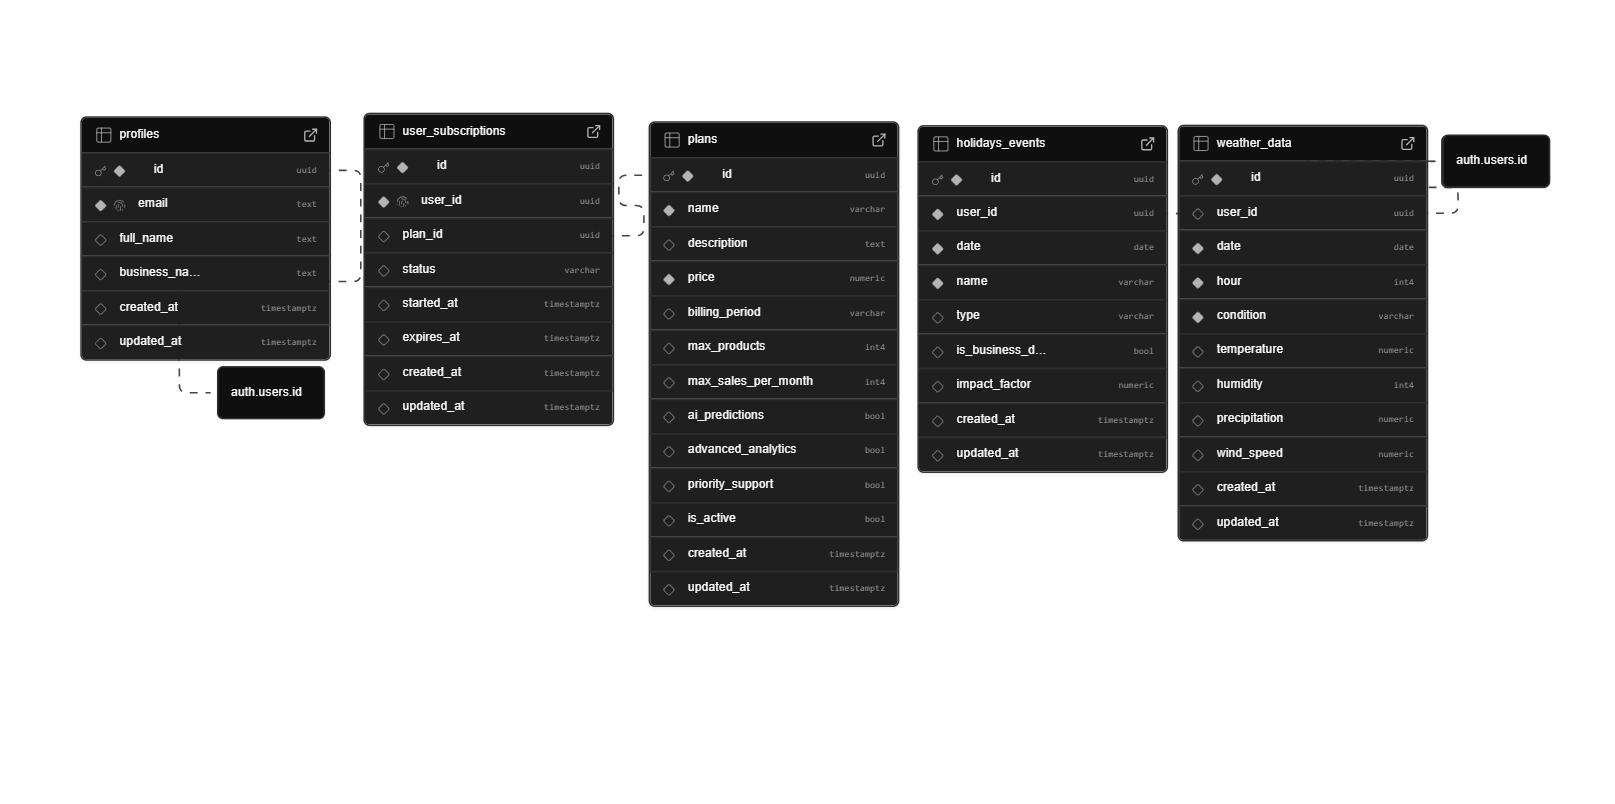
\includegraphics[width=0.95\textwidth]{images/ArquitecturaDB1.png} % <-- reemplazar por tu archivo
  \caption{Modelo de datos de AIVA 1-- Fuente: elaboración propia.}
  \label{fig:arquitectura-db}
\end{figure}
\vspace{1cm}

\begin{figure}[!htbp]
    \centering
    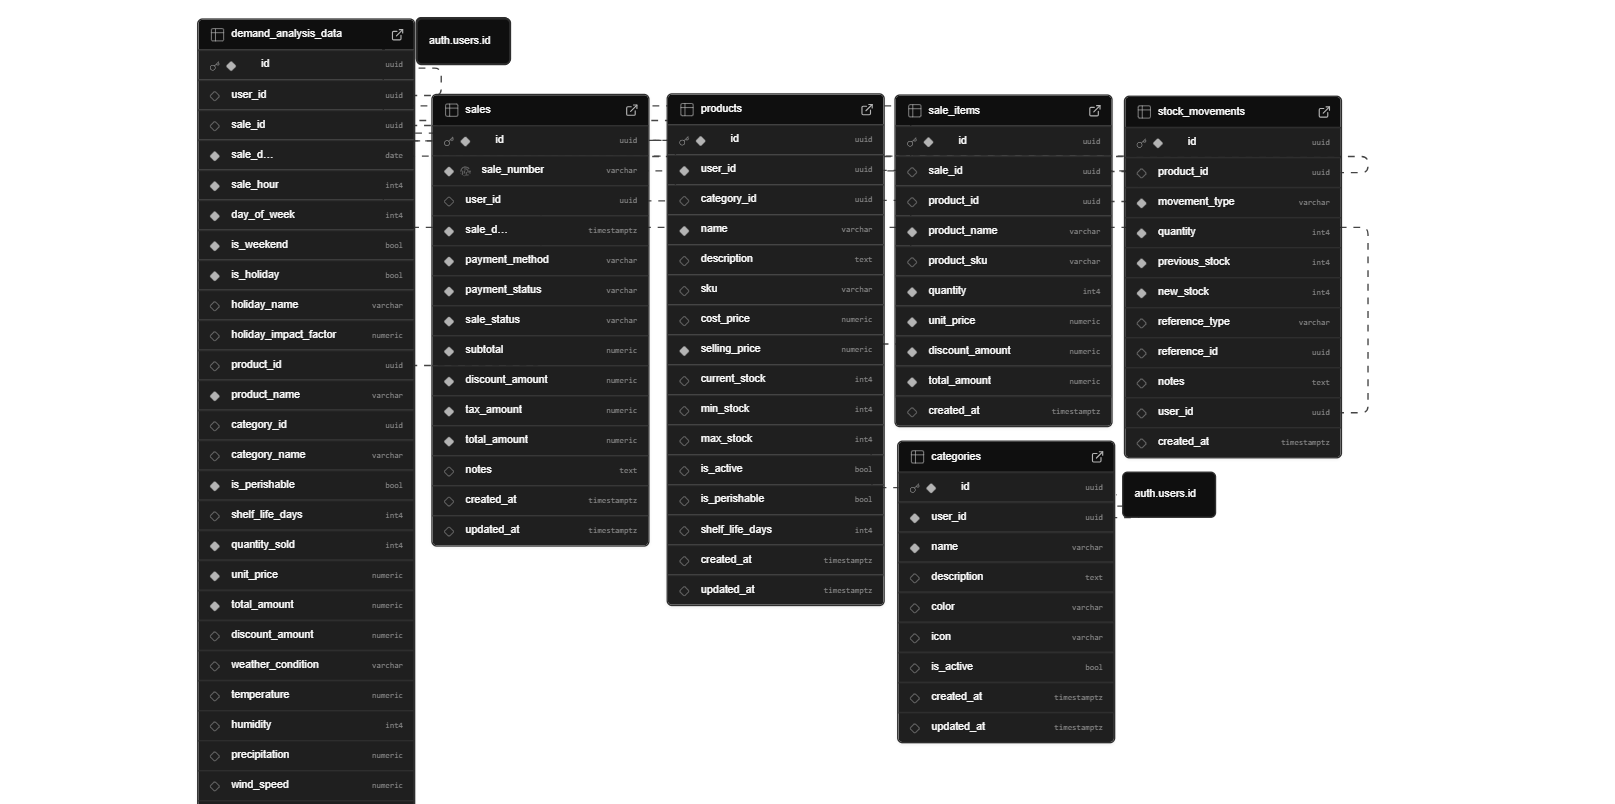
\includegraphics[width=0.95\textwidth]{images/ArquitecturaDB2.png} % <-- reemplazar por tu archivo
    \caption{Modelo de datos de AIVA 2-- Fuente: elaboración propia.}
    \label{fig:arquitectura-db2}
  \end{figure}
  \vspace{2cm}


\vspace{1cm}
\section{Diagrama de flujos}

Para describir el comportamiento dinámico del sistema incorporamos diagramas de flujo que muestran, paso a paso, cómo se procesan las operaciones clave. Estos esquemas complementan a los requerimientos y a la arquitectura estática, al hacer explícitas las secuencias, los puntos de decisión, los caminos alternativos y el manejo de errores, lo que facilita la validación funcional y el diseño de casos de prueba.


\subsection{DF-A · Autenticación}
El diagrama modela el control de acceso y el alta de usuarios. Se definió así para equilibrar seguridad (validaciones en el servicio de autenticación y verificación de correo), usabilidad (separación clara entre registro e inicio de sesión) y recuperabilidad (manejo de errores con retroalimentación inmediata). La convergencia final en el dashboard establece un único criterio de éxito y facilita la trazabilidad de estados; el objetivo es registrar las decisiones críticas del acceso sin describir pantallas intermedias.

\begin{figure}[!htbp]
  \centering
  \includegraphics[width=0.92\textwidth]{images/FlujoAutenticación.png}
  \caption{DF-A · Autenticación -- Fuente: elaboración propia}
  \label{fig:df-a-autenticacion}
\end{figure}


\subsection{DF-B · Carga de ventas}
El diagrama describe el proceso de registro de ventas desde dos orígenes complementarios: ingreso manual tipo POS y carga automática (OCR/CSV). Se define así para cubrir los escenarios operativos más frecuentes con validaciones progresivas y una confirmación explícita antes del alta, incorporando puntos de corrección para minimizar errores y preservar trazabilidad. La bifurcación temprana optimiza tiempos según la fuente de datos y el cierre en confirmación establece una única condición de éxito.

\begin{figure}[!htbp]
  \centering
  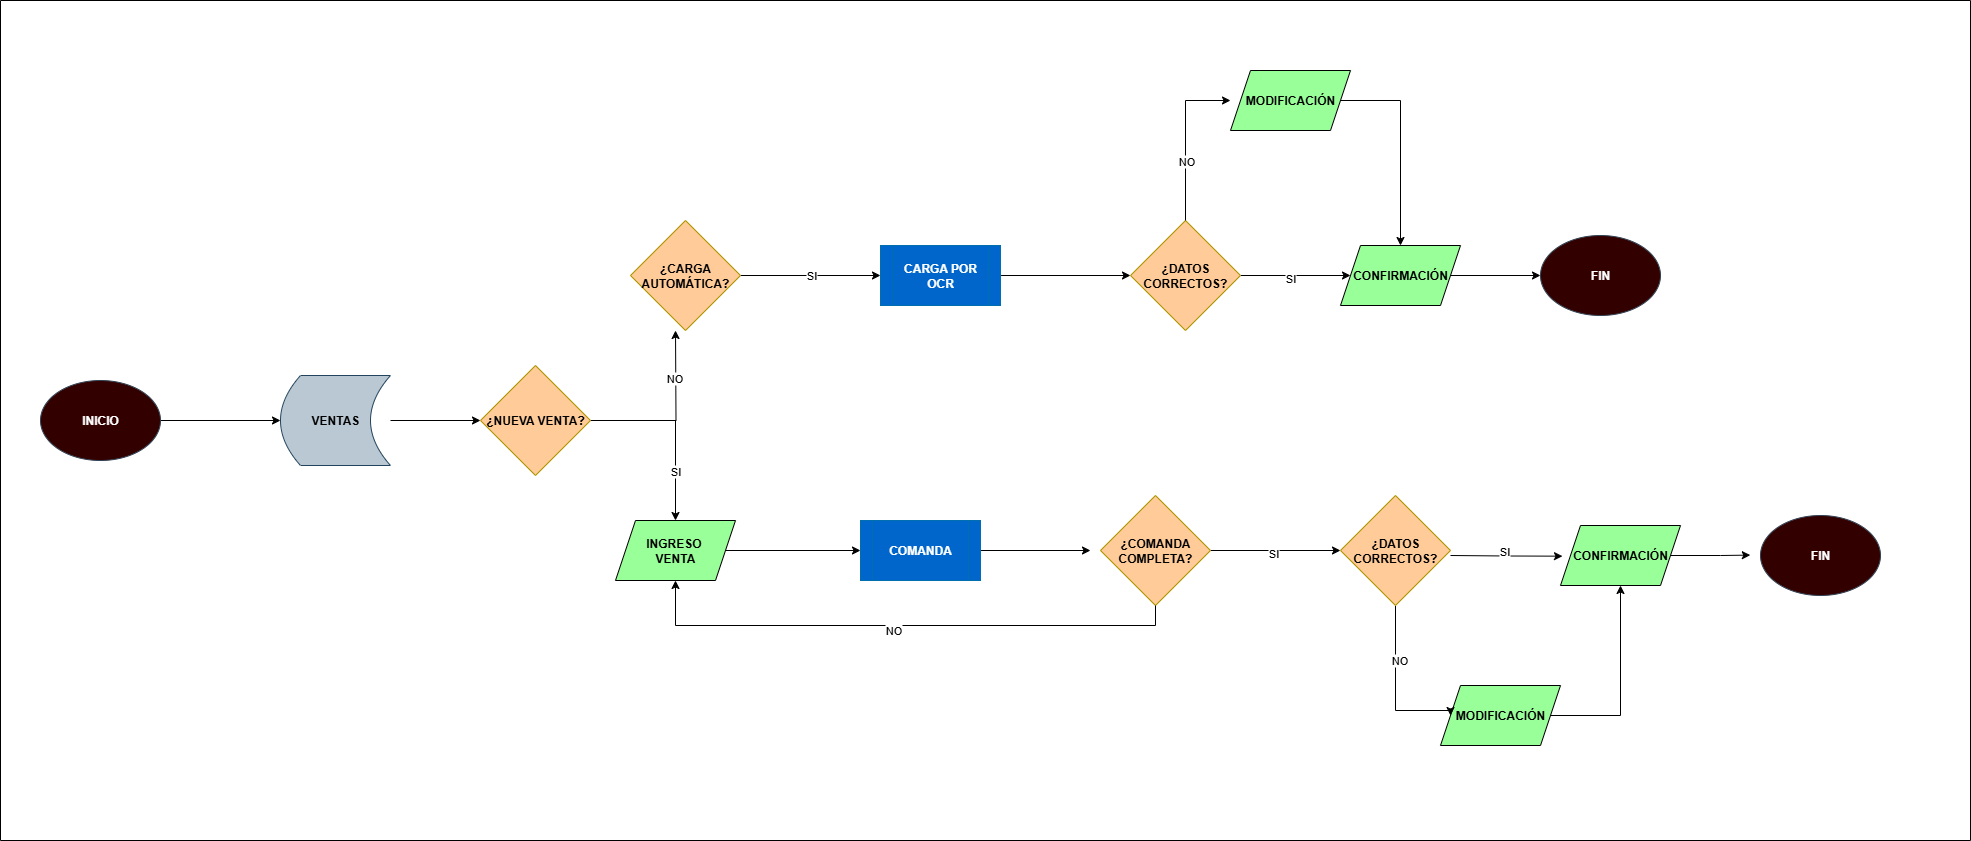
\includegraphics[width=0.92\textwidth]{images/FlujoVentas.drawio.png}
  \caption{DF-B · Carga de ventas -- Fuente: elaboración propia}
  \label{fig:df-b-ventas}
\end{figure}


\subsection{DF-C · Planes y suscripciones}
El diagrama describe la gestión de planes dentro de la aplicación. Al crear una cuenta, el usuario recibe automáticamente el plan gratuito; por este motivo, cualquier cambio de plan se realiza exclusivamente desde la app. El flujo contempla verificación de identidad y estado de suscripción, selección del nuevo plan y confirmación (incluida la validación de pago si corresponde). Ante éxito se actualiza la suscripción y se reflejan las capacidades en sesión; ante error se conserva el plan previo. El enfoque prioriza control de acceso, trazabilidad y una transición segura entre planes.

\begin{figure}[!htbp]
  \centering
  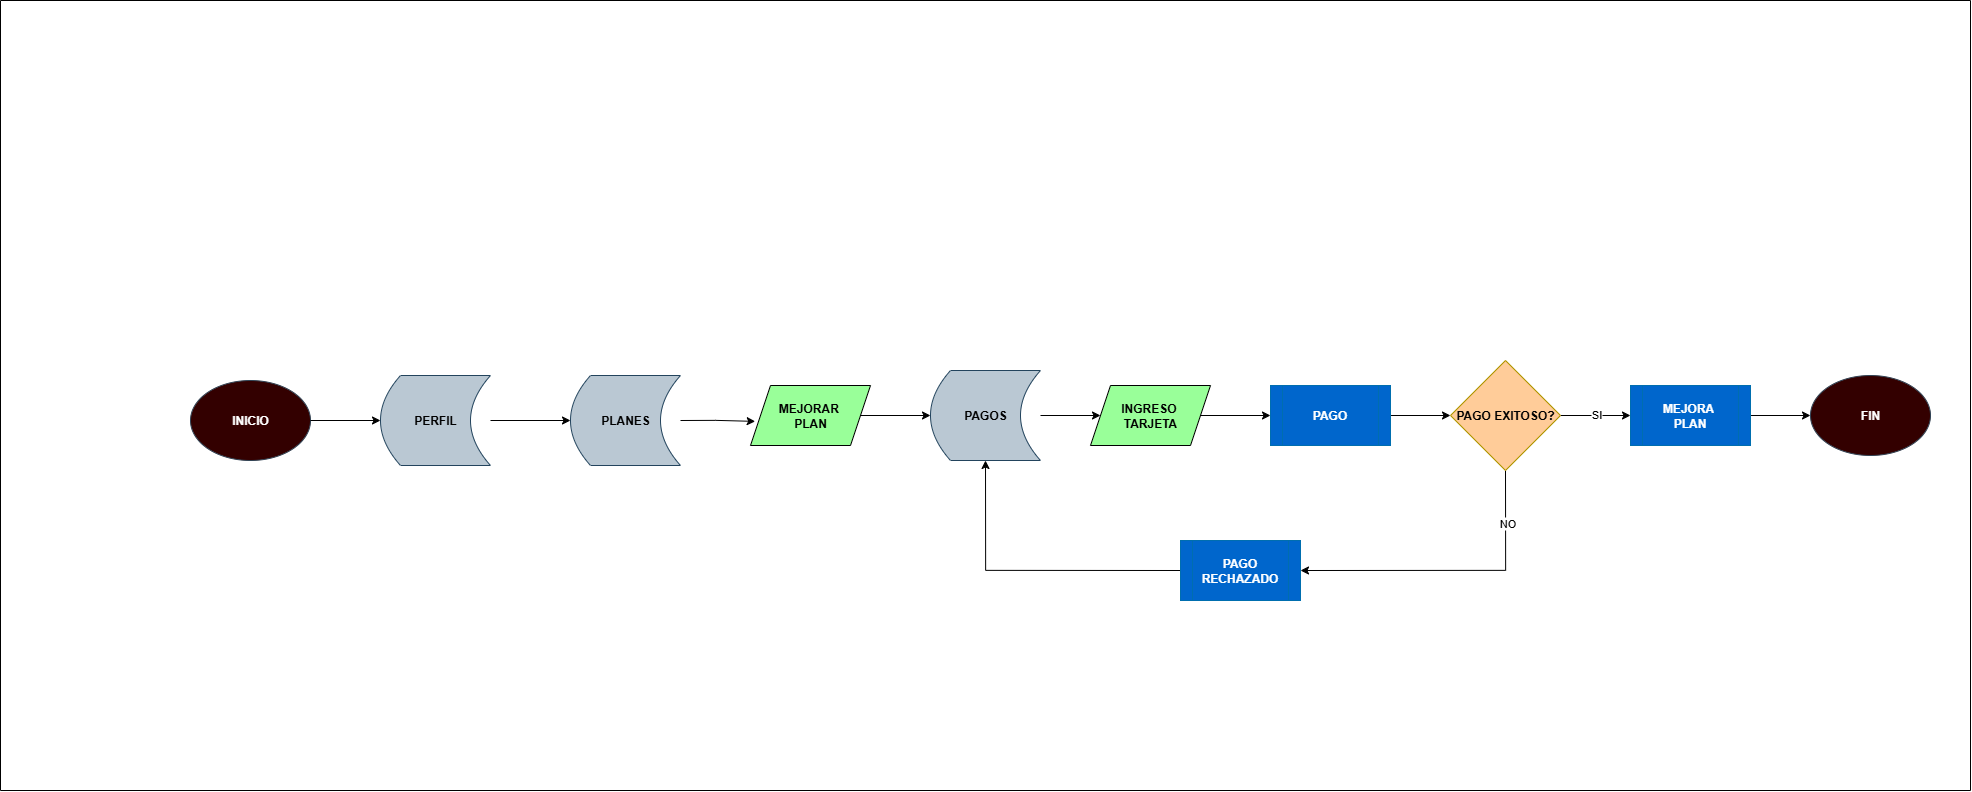
\includegraphics[width=0.92\textwidth]{images/FlujoPlanes.drawio.png}
  \caption{DF-C · Planes y suscripciones -- Fuente: elaboración propia}
  \label{fig:df-c-planes}
\end{figure}


\vspace{1cm}
\section{Identidad de marca}\label{sec:brand}

La identidad de marca de \textbf{AIVA} se diseñó para comunicar tecnología confiable, simplicidad operativa y foco en pequeños comercios. Esta sección documenta los elementos rectores de esa identidad y su relación con la experiencia de uso del sistema.

\subsection{Naming}
\textbf{AIVA} es un acrónimo de \textit{Asistente Inteligente para Ventas y Análisis}. El nombre cumple tres criterios: (i) \textit{memorabilidad} y pronunciación sencilla en español e inglés, (ii) \textit{brevedad} apta para interfaces y piezas breves (íconos, botones, navegación), y (iii) \textit{connotación} directa con analítica y apoyo a la decisión. El nombre se usa en mayúsculas para reforzar la legibilidad y la consistencia visual en la interfaz.

\subsection{Misión}
Poner la analítica predictiva al alcance de micro y pequeñas empresas de alimentos perecederos, reduciendo mermas y quiebres mediante planificación basada en datos. La misión orienta decisiones de producto hacia soluciones de bajo costo, fáciles de adoptar y con impacto operativo medible.

\subsection{Visión}
Constituirse en la plataforma de referencia en América Latina para la gestión de demanda en comercios de proximidad, integrando múltiples fuentes de datos (histórico, clima, calendario) y promoviendo prácticas sustentables de producción y reposición.

\subsection{Paleta de colores}\label{subsec:paleta}

La paleta cromática de \textbf{AIVA} fue definida para comunicar confianza tecnológica, claridad y foco en la toma de decisiones. El eje visual está compuesto por un rango de azules–índigo que se aplica en fondos y navegación, desde un índigo profundo hasta un azul más luminoso (\#1E2A78–\#3F6BFF). Esta base fría evoca precisión y estabilidad, atributos propios de una plataforma analítica, y refuerza la percepción de fiabilidad por parte del usuario.

Como acento de marca se incorpora el violeta (\#7C3AED, con su variante clara \#A78BFA), que introduce una connotación de innovación y modernidad. Este matiz se reserva para elementos de énfasis —botones primarios, indicadores destacados y piezas de comunicación—, logrando contraste visual sin perder coherencia con el tono profesional del sistema. Complementariamente, el cian (\#38BDF8) funciona como color informativo en enlaces y ayudas contextuales, guiando la atención sin distraer del contenido principal.

Los colores semánticos se emplean para codificar estados del sistema y facilitar la lectura operativa: el verde (\#22C55E) comunica confirmaciones y resultados positivos, mientras que el naranja (\#F59E0B) señala advertencias y situaciones que requieren seguimiento. La selección de saturación y brillo busca que estos mensajes sean perceptibles de forma inmediata, manteniendo, al mismo tiempo, una estética sobria adecuada al ámbito empresarial.

La familia de neutros se utiliza para garantizar legibilidad tipográfica y jerarquía en las superficies: un gris muy oscuro para textos (\#0F172A) y un gris claro para fondos (\#F1F5F9), complementados por blanco (\#FFFFFF) en componentes de alta claridad. En consonancia con pautas de accesibilidad, se privilegian combinaciones de alto contraste en las vistas más frecuentes, asegurando que la interfaz conserve nitidez tanto en entornos luminosos como en configuraciones de bajo brillo.

En conjunto, el gradiente principal de índigo a azul, el acento violeta y los semánticos verde/naranja construyen un lenguaje visual consistente: profesional en su base, expresivo en sus acentos y funcional en la comunicación de estados. Esta identidad cromática sostiene la experiencia de uso de AIVA y refuerza su posicionamiento como asistente inteligente para la gestión de demanda.

\begin{figure}[!htbp]
  \centering
  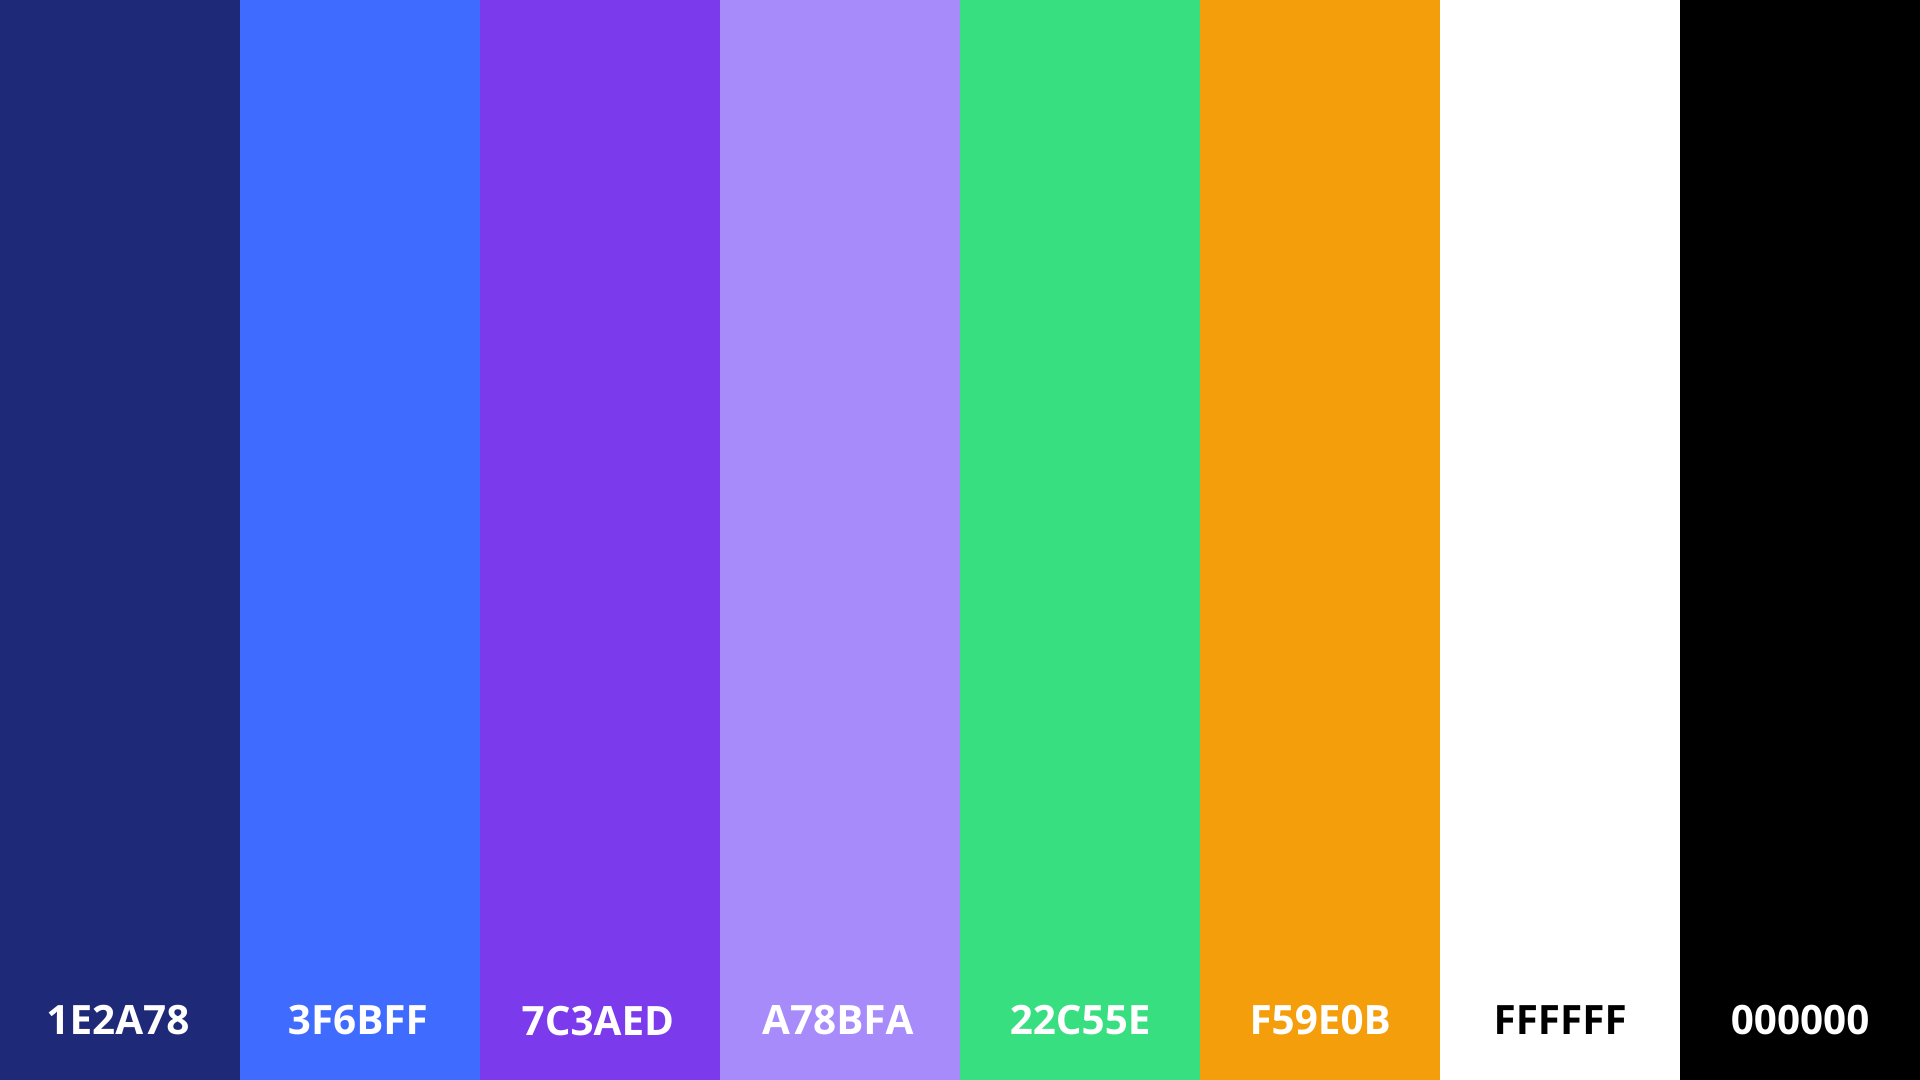
\includegraphics[width=0.92\textwidth]{images/paleta-aiva.png}
  \caption{Paleta de Colores -- Fuente: elaboración propia}
  \label{fig:paleta-aiva}
\end{figure}

\subsection{Logo}
El signo marcario combina un \textbf{símbolo geométrico} (módulos rectangulares que sugieren el trazo de una “A” y la idea de bloques de datos) con el \textbf{logotipo} “AIVA” en tipografía \textit{sans serif} de alta legibilidad.

\begin{itemize}
    \item \textbf{Configuración principal (lockup).} Símbolo a la izquierda y logotipo a la derecha, alineados sobre la línea base. El conjunto se utiliza en positivo (blanco) sobre fondos índigo/azules o en negativo (índigo/violeta) sobre fondos claros.
    \item \textbf{Área de protección.} Se mantiene un margen libre alrededor del logo equivalente a la altura del símbolo para evitar interferencias con otros elementos.
    \item \textbf{Tamaños mínimos.} Se asegura que el ancho total no sea inferior a 24\,mm en impresos (o 160\,px en pantalla) para conservar la legibilidad de las formas internas.
    \item \textbf{Variantes.} 
    \begin{itemize}
        \item \textit{Monocromo}: uso en una sola tinta (blanco o negro) cuando las restricciones de producción lo requieran.
        \item \textit{Isotipo}: sólo el símbolo para favicons, íconos de app o espacios reducidos.
    \end{itemize}
    \item \textbf{Usos incorrectos.} No distorsionar, rotar ni aplicar efectos de sombra; no alterar la paleta definida; no combinar el logo con fondos de bajo contraste que comprometan la lectura.
\end{itemize}

\vspace{1cm}

	\chapter{Conclusi\'on}\label{conclussions}

\section{Resumen de aportes}

Completar.

\section{Trabajo futuro}


Completar.

	\addcontentsline{toc}{chapter}{Bibliograf\'{\i}a}
	\printbibliography{}


	%\appendix
	%% TODO Esto no se agrega a la tesis debido al tiempo que llevaría. Cuando lo continúe, considerar que hay que cambiar la regla If_\X por la nueva, la proyección por la nueva, y modificar el casting para que tenga en cuenta el ket genérico. También reever los saltos de línea y los cortes de línea.

\chapter{Título del apéndice}\label{appendixA}

Contenido del apéndice.
	\newpage
	\listoffigures
	\newpage
	\listoftables
\end{document}
